\documentclass[11pt, a4paper]{article}

\usepackage[top=3.5cm, left=3.5cm, right=3.0cm, bottom=3.0cm, includehead, includefoot]{geometry}%margem 
\usepackage[]{graphicx} 
\usepackage{amssymb,amsmath}
%\usepackage[brazilian]{babel}
\usepackage[utf8]{inputenc}
\usepackage[square, numbers, comma, sort&compress]{natbib}
\usepackage{microtype}
\usepackage{siunitx}
\usepackage{cite}%bibliografia
%\usepackage{indentfirst} %espaço primeiro parágrafo
%\setlength{\parindent}{0cm} %parágrafo 1,25cm
%\setlength{\parskip}{0.5\baselineskip}

\usepackage{caption}
\usepackage{float} %posicionar figuras
\usepackage[font=scriptsize]{caption}
\usepackage[font=scriptsize]{subcaption} %legenda de figuras

\usepackage{epstopdf}

\DeclareMathSizes{5}{5}{5}{5}

\usepackage{subcaption}
\usepackage{booktabs}
\usepackage{fixltx2e} 
\usepackage{multirow}
\usepackage{array}
\usepackage{adjustbox}
\usepackage{wrapfig}
%\usepackage{breqn}
\usepackage{color}

\usepackage{rotating}

\usepackage{fancyhdr}
\pagestyle{fancy}
\rfoot{\copyright Nasser Alkmim}
\lfoot{2015}
\lhead{\leftmark}
\rhead{\thepage}
\cfoot{}
\renewcommand{\headrulewidth}{0pt}
\renewcommand{\footrulewidth}{0pt}

\usepackage{multicol}

\usepackage{psfrag}
\usepackage[pdfstartview=FitH,backref,colorlinks,bookmarksopen,urlcolor=black,linkcolor=black]{hyperref}


\font\ursymbol=psyr at 9pt % You also use other font sizes.
\def\urpartial{\mbox{\ursymbol\char"B6}}

%\usepackage{titlesec}
%\titlespacing{\section}{0cm}{.5cm}{.5cm}
%\titlespacing{\subsection}{0cm}{.5cm}{.5cm}
%\titlespacing{\subsubsection}{0cm}{.5cm}{.5cm}

\numberwithin{equation}{section} 

\usepackage{chngcntr}

\counterwithin{figure}{section}

%\usepackage{empheq}
%\newcommand*\widefbox[1]{\fbox{\hspace{2em}#1\hspace{2em}}}

\usepackage{tikz}
\usetikzlibrary{shapes,arrows}
\tikzstyle{block} = [rectangle, draw, 
    text width=5em, text centered, rounded corners, minimum height=2em]
\tikzstyle{line} = [draw, -latex']


\begin{document}

\begin{titlepage}
\vspace*{\fill}
 \begin{center}
 	
\includegraphics[scale=.3]{fig/logo7.eps}
    \end{center}
\vspace*{\fill}
\end{titlepage}



\thispagestyle{empty}
%\begin{abstract}

%\end{abstract}

\clearpage
\thispagestyle{empty}
\tableofcontents


\clearpage
\pagestyle{fancy}





\section{Indicial Notation}

The indicial notation will be used throughout this report. The indexes are going to indicate that the equation is true for a range ${1,2,3}$ for each index.

An extra convention will be added to include the natural coordinate system on the isoparametric space. It is well known that for the Cartesian coordinate system the derivatives with respect the spatial variables can be expressed with the comma convention,
\begin{equation}
T{,i} = \left[ \dfrac{\partial T}{\partial x_1}, \dfrac{\partial T}{\partial x_2}, \dfrac{\partial T}{\partial x_3} \right].
\end{equation}
Because the change in coordinate system is used in the finite elements implementation process, it's necessary to evaluate partial derivatives in the new system. The convention adopted here is to use capitalized indexes to express partial derivatives in the isoparametric space with respect to its spatial variables, $\xi$. Therefore,
\begin{equation}
T_{,I} = \left[ \dfrac{\partial T}{\partial \xi_1}, \dfrac{\partial T}{\partial \xi_2}, \dfrac{\partial T}{\partial \xi_3} \right].
\end{equation}

\section{Linear Elastic Mechanics}

The structural analysis consist in define a equilibrium equation for the system, a kinematic relation that relates the degree's of freedom movement with the elements deformation and a force-deformation relation for the element.

\subsection{Equilibrium}

The linearity means that the material behaves in a linear manner, therefore, all its strain energy is recoverable and the stress varies linearly with the strain.

In the theory formulation it is also assumed that the displacements are small. This assumption allow us to analyze the object on its undeformed configuration, ignoring nonlinear effects.

The governing equation for the structural domain is the linearized motion equation,
\begin{equation}
\boldsymbol \nabla \boldsymbol \cdot \boldsymbol \sigma + \mathbf{f}= 0.
\end{equation}
This equation is the equilibrium of a differential element inside the body. The divergence of stress represents the difference on each direction of the stress components, therefore the change is stress across a differential element must be equal to the force per unit volume in the correspondent direction. The same equation can be expressed with indicial notation,
\begin{equation}
\sigma_{ij,j} + f_i = 0
\end{equation}

\subsection{Kinematics}
The strain-displacement in its linearized form can be expressed as,
\begin{equation}
\varepsilon_{ij} = \dfrac{1}{2} (u_{i,j} + u_{j,i}),
\end{equation}
where $u_{i}$ is the displacement vector. This expression results from the analysis of the deformation on a infinitesimal element, assuming that when the elements deforms the deformed length can be approximated to its original configuration. The axial components are simply the rate of displacement on each direction,
\begin{align*}
\varepsilon_{11} &= u_{1,1}\\
\varepsilon_{22} &= u_{2,2}\\
\varepsilon_{33} &= u_{3,3}.
\end{align*}
The shear components are approximations for small changes in angles between the infinitesimal element sides. The notation $\varepsilon_{12}$ means the angular deformation between axis $x_1$ and $x_2$. Approximating the angle of rotation by the tangent assuming small deformations the strain between axis $x_1$ and $x_2$ is composed by a rotation on the $x_1$ axis due a vertical $u_2$ displacement, so $u_{2,1}$, and a rotation on the $x_2$ axis due a horizontal displacement $u_1$, therefore $u_{1, 2}$. Summing up both of the rotations we get,
\begin{align*}
\varepsilon_{12} &= u_{2,1} + u_{1,2} \\
\varepsilon_{13} &= u_{3,1} + u_{1,3} \\
\varepsilon_{23} &= u_{3,2} + u_{2,3}.
\end{align*}
The result is analogous for the other 2 planes.

\subsection{Constitutive Relation}
A constitutive relation can be expressed as a mapping of the deformation gradient, strains, to the stress tensor. There is a unique relation between the stress at a material point and the current local deformation,
\begin{equation}
\boldsymbol T =\boldsymbol  f(\boldsymbol F),
\end{equation}
where $\boldsymbol T$ is the Cauchy stress tensor, $\boldsymbol f$ is the mapping function which is does not depend of the position for homogeneous materials (same properties on every point) and $\boldsymbol F$ is the deformation gradient tensor.

The principal of material frame-indifference,
\begin{equation}
\boldsymbol f (\boldsymbol Q \cdot \boldsymbol F) = \boldsymbol Q \cdot \boldsymbol f(\boldsymbol F)\cdot \boldsymbol Q^T
\end{equation}

There are many equivalent forms of the constitutive relation, each form will have restrictions due the principle of material frame-indifferenc. One of the forms is the the second Piola-Kirchhoff stress tensor $\tilde{\boldsymbol S}$ as a function of the Green-St. Venant strain tensor $\boldsymbol E$.

The constitutive relation of the material relates the material parameters for stress and strain.
\begin{equation}
\sigma_{ij} = \mathbb{C}_{ijk\ell} \, \varepsilon_{k\ell},
\end{equation}
where the stress is related to the strain by a fourth order tensor. The stiffness tensor, $\mathbb{C}_{ijk\ell} $ is expressed by,
\begin{equation}
\mathbb{C}_{ijk\ell} = \lambda \; \delta_{ij} \delta_{k\ell} + 2 \mu \;
 \dfrac{1}{2} (\delta_{ik} \delta_{j\ell} + \delta_{i\ell} \delta_{jk}),
\end{equation}
where $\delta_{ij}$is the Kronecker delta. The $\lambda$ and $\mu$ are known as Lam$\acute{\text{e}}$ constants. This constants are related with the Young's modulus and Poisson ratio by, 
\begin{equation*}
\lambda = \dfrac{E \nu}{(1+\nu)(1-2\nu)}, \qquad \mu = \dfrac{E}{2(1+\nu)}.
\end{equation*}
Expressing the stress as function of displacements we get,
\begin{align*}
\sigma_{ij} &= \mathbb{C}_{ijk\ell} \, \varepsilon_{k\ell} \\
&=\mathbb{C}_{ijk\ell} \, \frac{1}{2} ( u_{k,\ell} + u_{\ell,k}) \\
&=  \mathbb{C}_{ijk\ell} \,  u_{k,\ell} \qquad (\text{Due symetry }\mathbb{C}_{ijk\ell} =\mathbb{C}_{ij\ell k}).
\end{align*}
For an Isotropic material the stress and strain are related by,
\begin{align*}
&\varepsilon_{11} = \dfrac{1}{E} [\sigma_{11} - \nu (\sigma_{22}+\sigma_{33})], &\varepsilon_{12} = \dfrac{1 + \nu}{E} \sigma_{12} \\
&
\varepsilon_{22} = \dfrac{1}{E} [\sigma_{22} - \nu (\sigma_{11}+\sigma_{33})], & \varepsilon_{13} = \dfrac{1 + \nu}{E} \sigma_{13}\\&
\varepsilon_{33} = \dfrac{1}{E} [\sigma_{33} - \nu (\sigma_{22}+\sigma_{11})], & 
\varepsilon_{23} = \dfrac{1 + \nu}{E} \sigma_{23}
\end{align*}
this way the constitutive relation consists of a system of 6 equations and the stiffness tensor can be viewed as a 6x6 matrix. In general, the reasons for that simplification are:
\begin{itemize}
\item[•] Because the stress tensor must be symmetric in order to satisfy angular equations of motion then the elasticity tensor must be symmetric as well on the same stress indexes, $\mathbb{C}_{ij\ell k} = \mathbb{C}_{ji\ell k}$. This symmetry reduces the number of independent entries on the elasticity tensor from $3^4 = 81$ to $6\cdot3\cdot3=54$.
\item[•] The property of the stiffness tensor of skew-symmetry with the symmetry by construction of the strain tensor require the stiffness tensor to be symmetry with the last two indexes, so $\mathbb{C}_{ij k\ell} = \mathbb{C}_{ij\ell k}$, therefore the number of independent entries goes to $6 \cdot 6 = 36$.
\item[•] For a hyperelastic material,  $\mathbb{C}_{ijk\ell}=\mathbb{C}_{k\ell ij }  $, reducing the independent stiffness component to $\frac{1}{2}(6 \cdot6+6)=21$. Which is equal to the number of independent entries on a symmetric 6x6 matrix.
\item[•] For a isotropic material, the independent components reduce to 2: the Young's modulus and the Poisson's ratio.
\end{itemize} 


\subsection{Weak Form}

Defining the solution space $\mathcal{U}$ and the space of trial (or weighting) function $\mathcal{V} $ as,

\begin{align*}
\mathcal{U} &= \{ u_i \;|\; u_i= u_i^d \quad \text{at} \quad x_i \in \partial \Omega^D \} \\
\mathcal{V} &= \{ w_i \;|\; w_i = 0 \quad \text{at} \quad x_i \in \partial \Omega^D \}
\end{align*}
which define a solution that satisfies the Dirichlet boundary conditions at $\partial \Omega^D$ and defined a set of allowable weighting functions that equals zero at the boundary where the Dirichlet condition is specified.

The weak formulation is obtained by multiplying the equation on both sides by $w_i$. The problem can be stated as find $u_i$ on $\mathcal{U}$ such that,
\begin{align*}
&
\sigma_{ij,j} + f_i = 0 \\
&
\int_{\Omega}w_i \sigma_{ij,j} \, \mathrm{d}\Omega + \int_{\Omega} w_i f_i \, \mathrm{d}\Omega = 0\\
&
\int_\Omega w_{i,j}  \sigma_{ij} \, \mathrm{d}\Omega
- \int_{\partial \Omega} w_i \sigma_{ij} n_j \, \mathrm{d}S+\int_\Omega w_i f_i \, \mathrm{d}\Omega = 0
\\&
\int_\Omega w_{i,j}  \sigma_{ij} \, \mathrm{d}\Omega
- \int_{\partial \Omega} w_i \bar{t}_i \, \mathrm{d}S+\int_\Omega w_i f_i \, \mathrm{d}\Omega = 0
\end{align*}
where, $\bar{t}_i=\sigma_{ij}n_j$ is the traction vector. The Green's Theorem were also used, it says: $(w_i \sigma_{ij})_{,j} = w_{i,j}\sigma_{ij} + w_i \sigma_{ij,j}$. And finally the divergence theorem was used to transform the integral over the domain on the integral over its boundary. The traction should be specified on the boundary $\partial \Omega^N$, noting that $\partial \Omega = \partial \Omega^N \cup \partial \Omega^D$.




\subsection{Finite Element Approximation}

The finite element approximation starts with the definition of a subset of the solution space,
\begin{align*}
\mathcal{\tilde{U}} &= \{ u_i^h \;|\; u_i^h = u_i^d \quad \text{at} \quad x_i \in \partial \Omega^D \} \\
\mathcal{\tilde{V}} &= \{ w_i^h \;|\; w_i^h = 0 \quad \text{at} \quad x_i \in \partial \Omega^D \}
\end{align*}
where, the choice for $u_i$ is specific,
\begin{equation}
u^h_i = \sum_{K=1}^N \phi(x_i) d_i.
\end{equation}
The summation represents the division of the domain into elements. The nodes at this elements are numbered from 1 to $N$. The function $\phi$ is such that its value is equal one at the nodes and zero elsewhere, varying linearly from node to node for a element type with linear shape function (It could be any degree polynomial). The $d_i$ represents a constant for each degree of freedom. Same of this goes for the trial function,
\begin{equation}
w^h_i = \sum_{K=1}^N \phi(x_i) c_i.
\end{equation}

At this point we can specify the element type, the choice for this work was the quadrilateral, or simply quad, element. In order to simplify the analysis and implementation its better to consider the integrals on each element. So, the equation for over each element is,
\begin{equation}
\int_{\Omega^e} w_{i,j}  \sigma_{ij} \, \mathrm{d}\Omega
- \int_{\partial \Omega^e} w_i \bar{t}_i \, \mathrm{d}S+\int_{\Omega^e} w_i f_i \, \mathrm{d}\Omega = 0.
\end{equation}

\subsection{Isoparametric Formulation}

The $\phi(x_i)$ function for each element, usually, are not actual formed in the Cartesian coordinates, instead they are represented as a function of the isoparametric coordinates $(e_I)$. Parametric because the mapping is giving by parameters, or the position is giving in term of parameters. Iso because the mapping is done using the same shape functions $\phi$. The functions for each element are giving by,
\begin{align*}
\phi^1 = \dfrac{1}{4} (1-\xi_1)(1-\xi_2) \qquad \phi^2 = \dfrac{1}{4} (1 + \xi_1)(1-\xi_2) \\
\phi^3= \dfrac{1}{4} (1+\xi_1)(1+\xi_2) \qquad \phi^4 = \dfrac{1}{4} (1 - \xi_1)(1+\xi_2).
\end{align*}


\subsubsection{Mapping Function}

We can define the mapping $\mathbf{G}$ which is expressed by,
\begin{equation*}
\mathbf{G(\xi_I)} = x_i(\xi_I) =
\begin{bmatrix}
x_1 (\xi_I) \\
x_2 (\xi_I)
\end{bmatrix} = 
\begin{bmatrix}
X_1^1 \phi^1 + X_1^2 \phi^2+ X_1^3 \phi^3 + X_1^4 \phi^4 \\[0.2cm]
X_2^1 \phi^1 + X_2^2 \phi^2+ X_2^3 \phi^3 + X_2^4 \phi^4 \\
 \end{bmatrix} = \sum_{A=1}^4
X^A_i \phi^A
\end{equation*}
Here, the superscript is used to distinct itself from the subscript that marks the presence of multiple degree's of freedom. The explicit summation is used to not confuse with the Einstein summation over the degree's of freedom. There is four terms in the summation because there are four different shape functions for each element. The $X_i$ represents the nodes coordinates in the Cartesian system. The mapping means that coordinates in the Cartesian system are function of the coordinates in the Isoparametric system, $x_i = x_i(\xi_I)$.

\subsubsection{Shape Function's Gradient}

The gradient of the basis functions for 2 dimensions is given by,
\begin{equation*}
\phi^a_{,i} =  \dfrac{\partial \phi^a}{\partial x_i} = 
\begin{bmatrix}
\dfrac{\partial \phi^a}{\partial x_1}  & \dfrac{\partial \phi^a}{\partial x_2} 
\end{bmatrix}=
\begin{bmatrix}
\phi^a_{,1} & \phi^a_{,2}
\end{bmatrix} 
\end{equation*}
mapping from isoparametric to Cartesian with,
\begin{equation*}
\mathbf{x} = ( x_1, x_2) = \mathbf{G}(\boldsymbol \xi) = \mathbf{G} (\xi_1, \xi_2) = \mathbf{x}(\boldsymbol \xi) = (x_1(\xi_1,\xi_2), x_2(\xi_1,\xi_2))
\end{equation*}
We can find the gradient of the basis functions in the isoparametric coordinate system,
\begin{align*}
\dfrac{\partial \phi^a(x_i)}{\partial \xi_I} &=\dfrac{\partial \phi^a( \mathbf{G}( \xi_I))}{\partial \xi_I}  \\
&= \dfrac{\partial \phi^a}{\partial \xi_I}
\dfrac{\partial \xi_I}{\partial x_i} \\
& = \dfrac{\partial \phi^a}{\partial \xi_1}
\dfrac{\partial \xi_1}{\partial x_i} +
\dfrac{\partial \phi^a}{\partial \xi_2}
\dfrac{\partial \xi_2}{\partial x_i} \\
&= \begin{bmatrix}
\dfrac{\partial \phi^a}{\partial \xi_1}
\dfrac{\partial \xi_1}{\partial x_1} +
\dfrac{\partial \phi^a}{\partial \xi_2}
\dfrac{\partial \xi_2}{\partial x_1} \\[0.4cm]
\dfrac{\partial \phi^a}{\partial \xi_1}
\dfrac{\partial \xi_1}{\partial x_2} +
\dfrac{\partial \phi^a}{\partial \xi_2}
\dfrac{\partial \xi_2}{\partial x_2} 
\end{bmatrix} \\
&= 
\begin{bmatrix}
\dfrac{\partial \xi_1}{\partial x_1} & \dfrac{\partial \xi_2}{\partial x_1}\\[0.4cm]
\dfrac{\partial \xi_1}{\partial x_2} & \dfrac{\partial \xi_2}{\partial x_2}
\end{bmatrix}
\begin{bmatrix}
\dfrac{\partial \phi^a}{\partial \xi_1} \\[0.4cm] \dfrac{\partial \phi^a}{\partial \xi_2}
\end{bmatrix} \\
&= \phi^a_{,I} \xi_{I,i}
\end{align*}
where, the subscript $(,I)$ indicates partial derivative with respect the isoparametric variables $\xi_I$. 

\subsubsection{Jacobian}

The Jacobian matrix of the transformation is calculated as,
\begin{equation}
J_{iI} = x_{i,I} = \begin{bmatrix}
\dfrac{\partial x_1}{\partial \xi_1}  & \dfrac{\partial x_1}{\partial \xi_2} \\[0.4cm]
\dfrac{\partial x_2}{\partial \xi_1}  & \dfrac{\partial x_2}{\partial \xi_2} 
\end{bmatrix}
\end{equation}
which is the inverse of the matrix generated from the chain rule when the gradient was computed for shape functions,
\begin{equation}
\begin{bmatrix}
\dfrac{\partial x_1}{\partial \xi_1}  & \dfrac{\partial x_1}{\partial \xi_2} \\[0.4cm]
\dfrac{\partial x_2}{\partial \xi_1}  & \dfrac{\partial x_2}{\partial \xi_2} 
\end{bmatrix}^{-1}
=
\begin{bmatrix}
\dfrac{\partial \xi_1}{\partial x_1} & \dfrac{\partial \xi_2}{\partial x_1}\\[0.4cm]
\dfrac{\partial \xi_1}{\partial x_2} & \dfrac{\partial \xi_2}{\partial x_2}
\end{bmatrix}
\end{equation}
Then, because we already have a isoparametric mapping: $x_i=\sum_{A=1}^4 \phi^A \chi_i^A$ we can calculate the derivatives that compose the Jacobian matrix.
The basis function can be conveniently be rewrite in the following form,
\begin{equation}
\phi^A = \dfrac{1}{4} \left(1 + \chi^A_1 \xi_1\right)  \left(1 + \chi_2^A \xi_2\right) 
\end{equation}
where $\chi^A_i$ are the coordinate of the node in the natural (isoparametric) domain,
\begin{align*}
 \chi^1_i = (-1, -1) \qquad 
\chi^2_i = (1, -1) \\
\chi^3_i = (1, 1) \qquad \chi_i^4 = (-1, 1)
\end{align*}
the position in the real domain becomes,
\begin{equation}
x_i (\xi_I) =   \sum_{A=1}^4 X_i^A \dfrac{1}{4} \left(1 + \chi_1^A \xi_1\right) \left(1 + \chi_2^A \xi_2\right) .
\end{equation}
The derivative of the position in the real domain with respect the natural coordinates can be expressed as,
\begin{align*}
\dfrac{\partial x_i}{\partial \xi_1} &= \sum_{A=1}^4 X_i^A \dfrac{1}{4} \chi_1^A \left( 1 + \chi_2^A \xi_2 \right) \\
\dfrac{\partial x_i}{\partial \xi_2} &= \sum_{A=1}^4 X_i^A \dfrac{1}{4} \left( 1 + \chi_1^A \xi_1 \right)  \chi_2^A 
\end{align*}
with that we can compute the Jacobian matrix. The nodes coordinates in the real domain, $X^A_i$ (each node $A=1,2,3,4$ for horizontal and vertical component $i=1,2$) and the nodes in the natural domain, $\chi_i^A$, are all known. We note that the derivatives will be function of $\xi_1$ or $\xi_2$. The inverse (useful for the chain rule derivatives) of a 2x2 matrix has a explicit formula:
\begin{equation}
J^{-1}_{ij} = \dfrac{1}{\det[J_{ij}]} \begin{bmatrix}
J_{22} & - J_{12} \\
 -J_{21} & J_{11}
\end{bmatrix} =
\dfrac{1}{\det[J_{ij}]}
\begin{bmatrix}
\dfrac{\partial x_2}{\partial \xi_2}  & -\dfrac{\partial x_1}{\partial \xi_2} \\[0.4cm]
-\dfrac{\partial x_2}{\partial \xi_1}  &  \dfrac{\partial x_1}{\partial \xi_1}
\end{bmatrix}
=
\begin{bmatrix}
\dfrac{\partial \xi_1}{\partial x_1} & \dfrac{\partial \xi_2}{\partial x_1}\\[0.4cm]
\dfrac{\partial \xi_1}{\partial x_2} & \dfrac{\partial \xi_2}{\partial x_2}
\end{bmatrix}
\end{equation}

\subsubsection{Line Integral Jacobian}

The change in coordinates for a line integral will require a ration between path lengths. Those ratios, Jacobian, are computed for each of the four sides of the element.
\begin{align*}
j=1 & \qquad J_s^1\; \mathrm{d} S  = \sqrt{\left(\dfrac{\partial x_1}{\partial \xi_2}\right)^2 + \left(\dfrac{\partial x_2}{\partial \xi_2}\right)^2}\, \mathrm{d} \xi_2 \qquad (\text{Evaluated at } \xi_1=1)
\\
j=2 & \qquad J_s^2\; \mathrm{d} S  =\sqrt{\left(\dfrac{\partial x_1}{\partial \xi_1}\right)^2 + \left(\dfrac{\partial x_2}{\partial \xi_1}\right)^2}\, \mathrm{d} \xi_1 \qquad (\text{Evaluated at } \xi_2=1)
\\
j=3 & \qquad J_s^3\; \mathrm{d} S = \sqrt{\left(\dfrac{\partial x_1}{\partial \xi_2}\right)^2 + \left(\dfrac{\partial x_2}{\partial \xi_2}\right)^2}\, \mathrm{d} \xi_2 \qquad (\text{Evaluated at } \xi_1=-1)
\\
j=4 & \qquad J_s^4\; \mathrm{d} S  = \sqrt{\left(\dfrac{\partial x_1}{\partial \xi_1}\right)^2 + \left(\dfrac{\partial x_2}{\partial \xi_1}\right)^2}\, \mathrm{d} \xi_1 \qquad (\text{Evaluated at } \xi_2=-1)
\end{align*}
Here, the element side where $\xi_i=1$ is said to be the first.


\subsection{Approximate Solution on the Weak Form}

Substituting the approximate solution for each element into the weak form, we get an matrix multiplication for each integral.

\subsubsection{Stiffness Matrix Integral}

First thing is to divide the domain into a collection of elements. Second, using the constitutive relation for stress-strain. Third, substitute the approximate solution.
\begin{align*}
\int_\Omega w_{i,j}  \sigma_{ij}\; \mathrm{d}\Omega &=
\sum_e \int_{\Omega^e} w_{i,j} \, \mathbb{C}_{ijk\ell}\, u_{k,\ell} \; \mathrm{d}\Omega
\\
&= 
\sum_e \int_{\Omega^e} \left( \sum_{A=1}^4 \phi^A_{,j} c_i^A \right)   \mathbb{C}_{ijk\ell} \left( \sum_{B=1}^4 \phi^B_{,\ell} d_k^B \right) \; \mathrm{d}\Omega
\\
&=
 \sum_e\sum_{A,B}^4  c_i^A \left( \int_{\Omega^e} \phi^A_{,j} \mathbb{C}_{ijk\ell} \;\phi^B_{,\ell}\; \mathrm{d} \Omega \right) d_k^B  \\
&= \sum_e\sum_{A,B}^4 c_i^A K_{ik}^{AB} d^B_k \\
&= \sum_e\sum_{A,B}^4 (\mathbf{c}^{A})^T \mathbf{K}^{AB} \mathbf{d}^B
\end{align*}
the stiffness matrix $\mathbf{K}$ is formed with the contraction of the fourth order elasticity tensor to a scalar. The contraction is obtained with the multiplication of the fourth order tensor by the second order from the left and from the right. It is good to notice that again all the subscripts represents the spatial variables in the Cartesian system (lower case). The vector $d_k^B$ has 8 components and the second the matrix $K_{ik}^{AB}$ is $8\;x\;8$. The second order tensors are the gradients of the basis functions. 

Using the change of variables, the stiffness matrix can be obtained by,
\begin{align*}
K_{ik}^{AB}
&=
\int_{\Omega^e} \phi^A_{,j} \mathbb{C}_{ijk\ell} \;\phi^B_{,\ell} \; \mathrm{d} \Omega \\
&= 
\int_{\Omega^e_\xi} \phi^A_{,I} \xi_{I,j}\; \mathbb{C}_{ijk\ell} \; \phi^B_{,I} \xi_{I,\ell} \det[x_{i,I}] \; \mathrm{d} \Omega
\end{align*}
where, $\Omega_{\xi}^e$ represents the element domain in the isoparametric space. All the terms of the integral should be evaluated using the the natural coordinate system.

\subsubsection{Load Vector Integral}

The load vector is obtained from the integral,
\begin{align*}
\int_\Omega w_i f_i \; \mathrm{d} \Omega 
&=
\sum_e \int_{\Omega^e} w_i f_i \; \mathrm{d} \Omega 
\\
&=
\sum_e \int_{\Omega^e} \left( \sum_{A=1}^4 \phi^A c_i^A \right)  f_i \; \mathrm{d} \Omega 
\\
&=
\sum_e \sum_{A=1}^4  c_i^A  \left( \int_{\Omega^e} \phi^A f_i \; \mathrm{d} \Omega \right)
\\
&=
\sum_e \sum_{A=1}^4  c_i^A F_i^A 
\\
&=
\sum_e \sum_{A=1}^4  (\mathbf{c}^A)^T \mathbf{F}^A
\end{align*}
changing the coordinates, the load vector for each element can be calculated by,
\begin{align*}
F_i^A &= \int_{\Omega^e} \phi^A f_i \; \mathrm{d} \Omega 
\\
&=
\int_{\Omega^e_\xi} \phi^A(\xi_I) f_i(\xi_I) \det[x_{i,I}] \; \mathrm{d} \Omega
\end{align*}
This integral is simpler than the stiffness one because there is no derivative of shape functions. We only need to use the mapping $x_i = x_i(\xi_I)$ to change the coordinate system and add the Jacobian.

\subsubsection{Traction Vector Integral}

The integral for the traction vector is the line integral over the domain boundaries,
\begin{align*}
\int_{\partial \Omega} w_i \bar{t}_i \; \mathrm{d} S
&=
\sum_e \int_{\partial \Omega^e} w_i \bar{t}_i \; \mathrm{d} S
\\
&=
\sum_e \int_{\partial \Omega^e} \left( \sum_{A=1}^4 \phi^A c_i^A \right) \bar{t}_i \; \mathrm{d} S
\\
&=
\sum_e \sum_{A=1}^4 c_i^A \left( \int_{\partial \Omega^e} \phi^A \bar{t}_i \; \mathrm{d} S\right)  
\\
&=
\sum_e \sum_{A=1}^4  c_i^A T_i^A 
\\
&=
\sum_e \sum_{A=1}^4  (\mathbf{c}^A)^T \mathbf{T}^A
\end{align*}

Changing the coordinate system for the isoparametric domain, we can calculate the Traction vector ($2\;x\;1$) for each node $A$ with,
\begin{align*}
T_i^A &=  \int_{\partial \Omega^e} \phi^A \bar{t}_i \; \mathrm{d} S 
\\
&=
\int_{\partial \Omega^e_\xi} \; \phi^A(\xi_I) \bar{t}_i(\xi_I) \det[J_s]\; \mathrm{d} S
\end{align*}
where, the boundary $\partial \Omega^e_\xi$ can be divided into 4 paths, $\Gamma^1, \Gamma^2, \Gamma^3, \Gamma^4$ referent to the element sides. Each side will have a different Jacobian.
\begin{align*}
T_i^A &= \sum_{j=1}^4 \int_{\Gamma^j} \;  \phi^A(\xi_I) \bar{t}_i(\xi_I) J_s^j \; \mathrm{d} S
\\
&=
\int_{\Gamma^1} \phi^A(1, \xi_2) \; \bar{t}_i(1, \xi_2) \sqrt{\left(\dfrac{\partial x_1}{\partial \xi_2}\right)^2 + \left(\dfrac{\partial x_2}{\partial \xi_2}\right)^2}\, \mathrm{d} \xi_2 
 \\ & \mathrel{\phantom{=}} +
\int_{\Gamma^2} \phi^A(\xi_1, 1) \; \bar{t}_i(\xi_1, 1) \sqrt{\left(\dfrac{\partial x_1}{\partial \xi_1}\right)^2 + \left(\dfrac{\partial x_2}{\partial \xi_1}\right)^2}\, \mathrm{d} \xi_1
 \\ &\mathrel{\phantom{=}} +
\int_{\Gamma^3} \phi^A(1, \xi_2)\;  \bar{t}_i(1, \xi_2) \sqrt{\left(\dfrac{\partial x_1}{\partial \xi_2}\right)^2 + \left(\dfrac{\partial x_2}{\partial \xi_2}\right)^2}\, \mathrm{d} \xi_2 
 \\& \mathrel{\phantom{=}} +
\int_{\Gamma^4} \phi^A(\xi_1, 1) \; \bar{t}_i(\xi_1, 1) \sqrt{\left(\dfrac{\partial x_1}{\partial \xi_1}\right)^2 + \left(\dfrac{\partial x_2}{\partial \xi_1}\right)^2}\, \mathrm{d} \xi_1
\end{align*}


\section{Implementation}

For implementation we write the multiplications inside the integral in matrix form. The integrals are calculated using Gaussian Quadrature so, all function are going to be previously evaluated at the Gauss Points (GP). 


\subsection{Mesh Generation}

The implementation of the mesh is done with two approachs, the first one a regular rectangular mesh and the second a general with any geometry. Both of the approach produce a mesh geometry with quadrilateral elements.


\begin{figure}[H]
\centering
	\begin{subfigure}[H]{0.49\textwidth}
		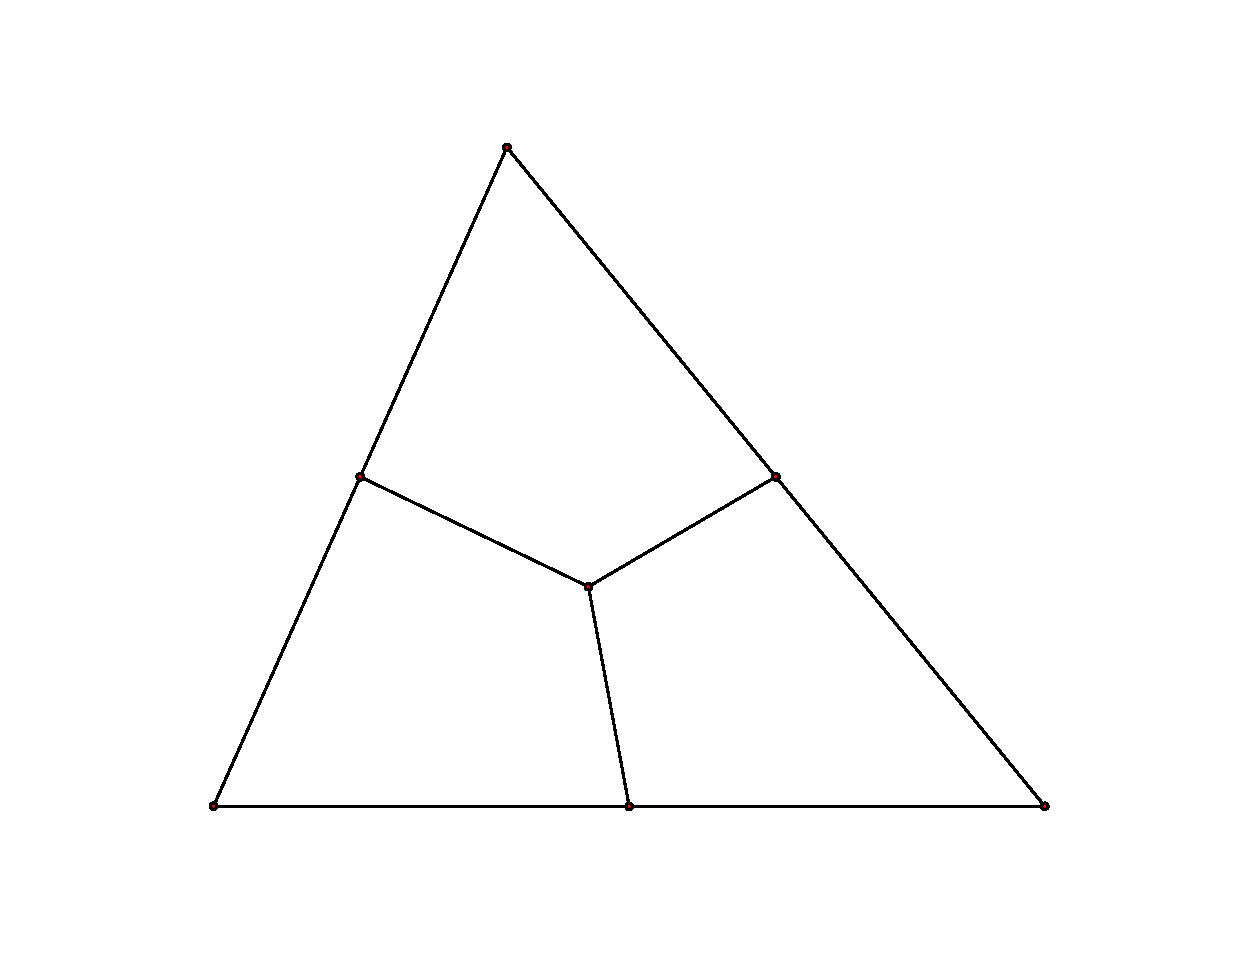
\includegraphics[width=1.2\textwidth]{fig/mesh1.eps}
		\caption{}
		\label{fig:1}
	\end{subfigure}
	\begin{subfigure}[H]{0.49\textwidth}
		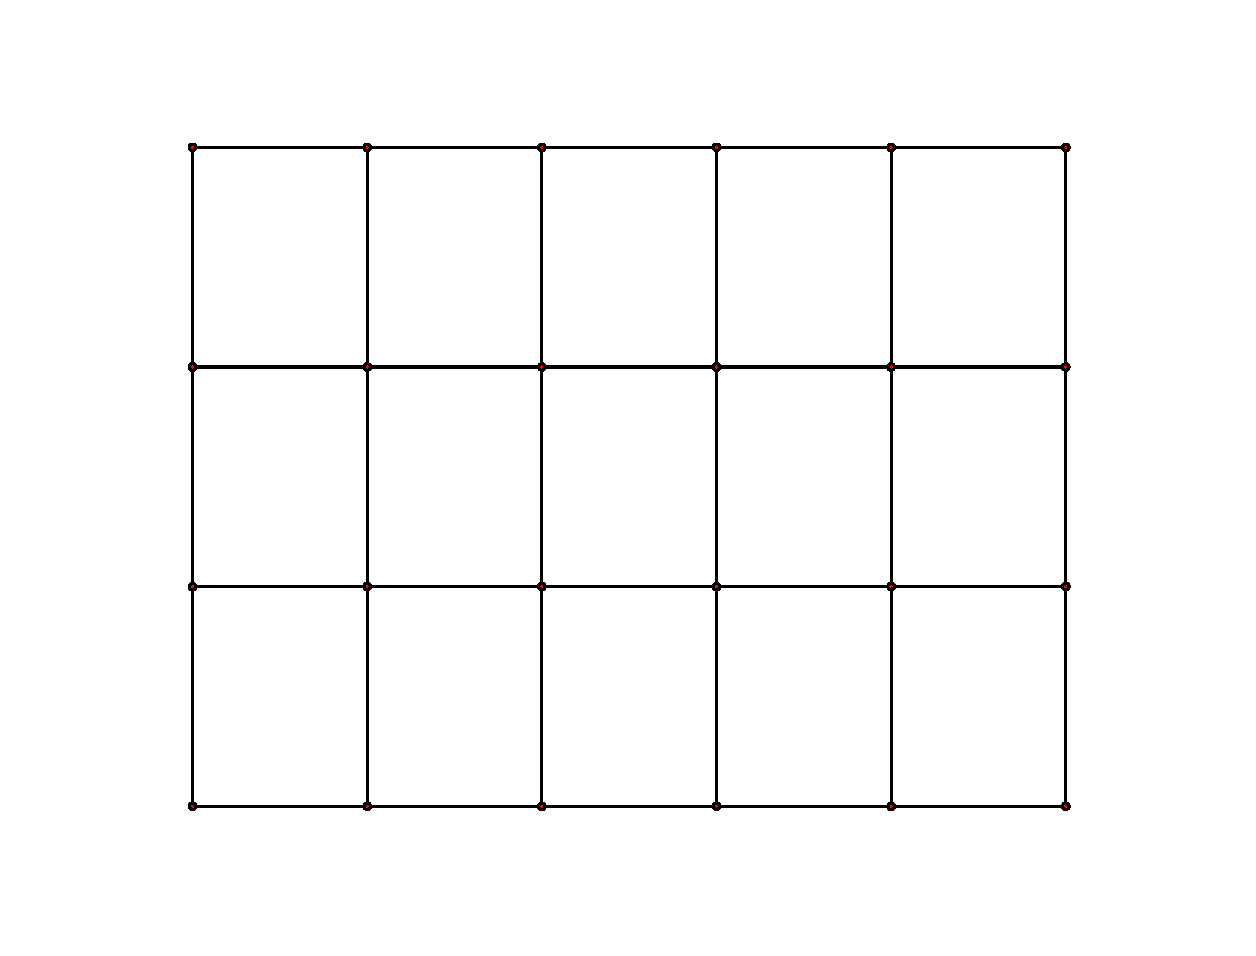
\includegraphics[width=\textwidth]{fig/mesh2.eps}
		\caption{}
		\label{fig:2}
	\end{subfigure}
	\caption{fig(a) is a general shape mesh and fig(b) is a regular rectangular mesh, both with quadrilateral elements.}
	\label{fig:3_1}
\end{figure}

The mesh is created as a module (a different file). The module has its attributes. The main attribute of the module is to instantiate a mesh geometry and its properties, then we can instantiate a regular mesh or a general shape. When a class instantiate something, an object is created. This object, mesh, contains attributes that can be used later.

The general shape mesh is created using Gmsh. Gmsh is copyright \copyright 1997-2014 by C. Geuzaine and J.-F. Remacle. Gmsh is a free to use software and can be distributed under the General Public License (GPL).

\subsubsection{Gmsh}

The first step for generate a mesh is to create the outside nodes. This is done by going to geometry, elementary entities, add, point. Then these points are connected with straight lines. The second step is to define a plane surface. Third is to create physical groups, lines for boundary conditions and surface that will generate a connectivity matrix for the elements. In order to get quad elements is necessary to specify on the mesh options (tools-options-mesh-general) that the subdivision algorithm is "All Quads". Finally the mesh is created by clicking on the 2D. The size of the elements can be adjusted later on the options menu.


\begin{figure}[H]
\centering
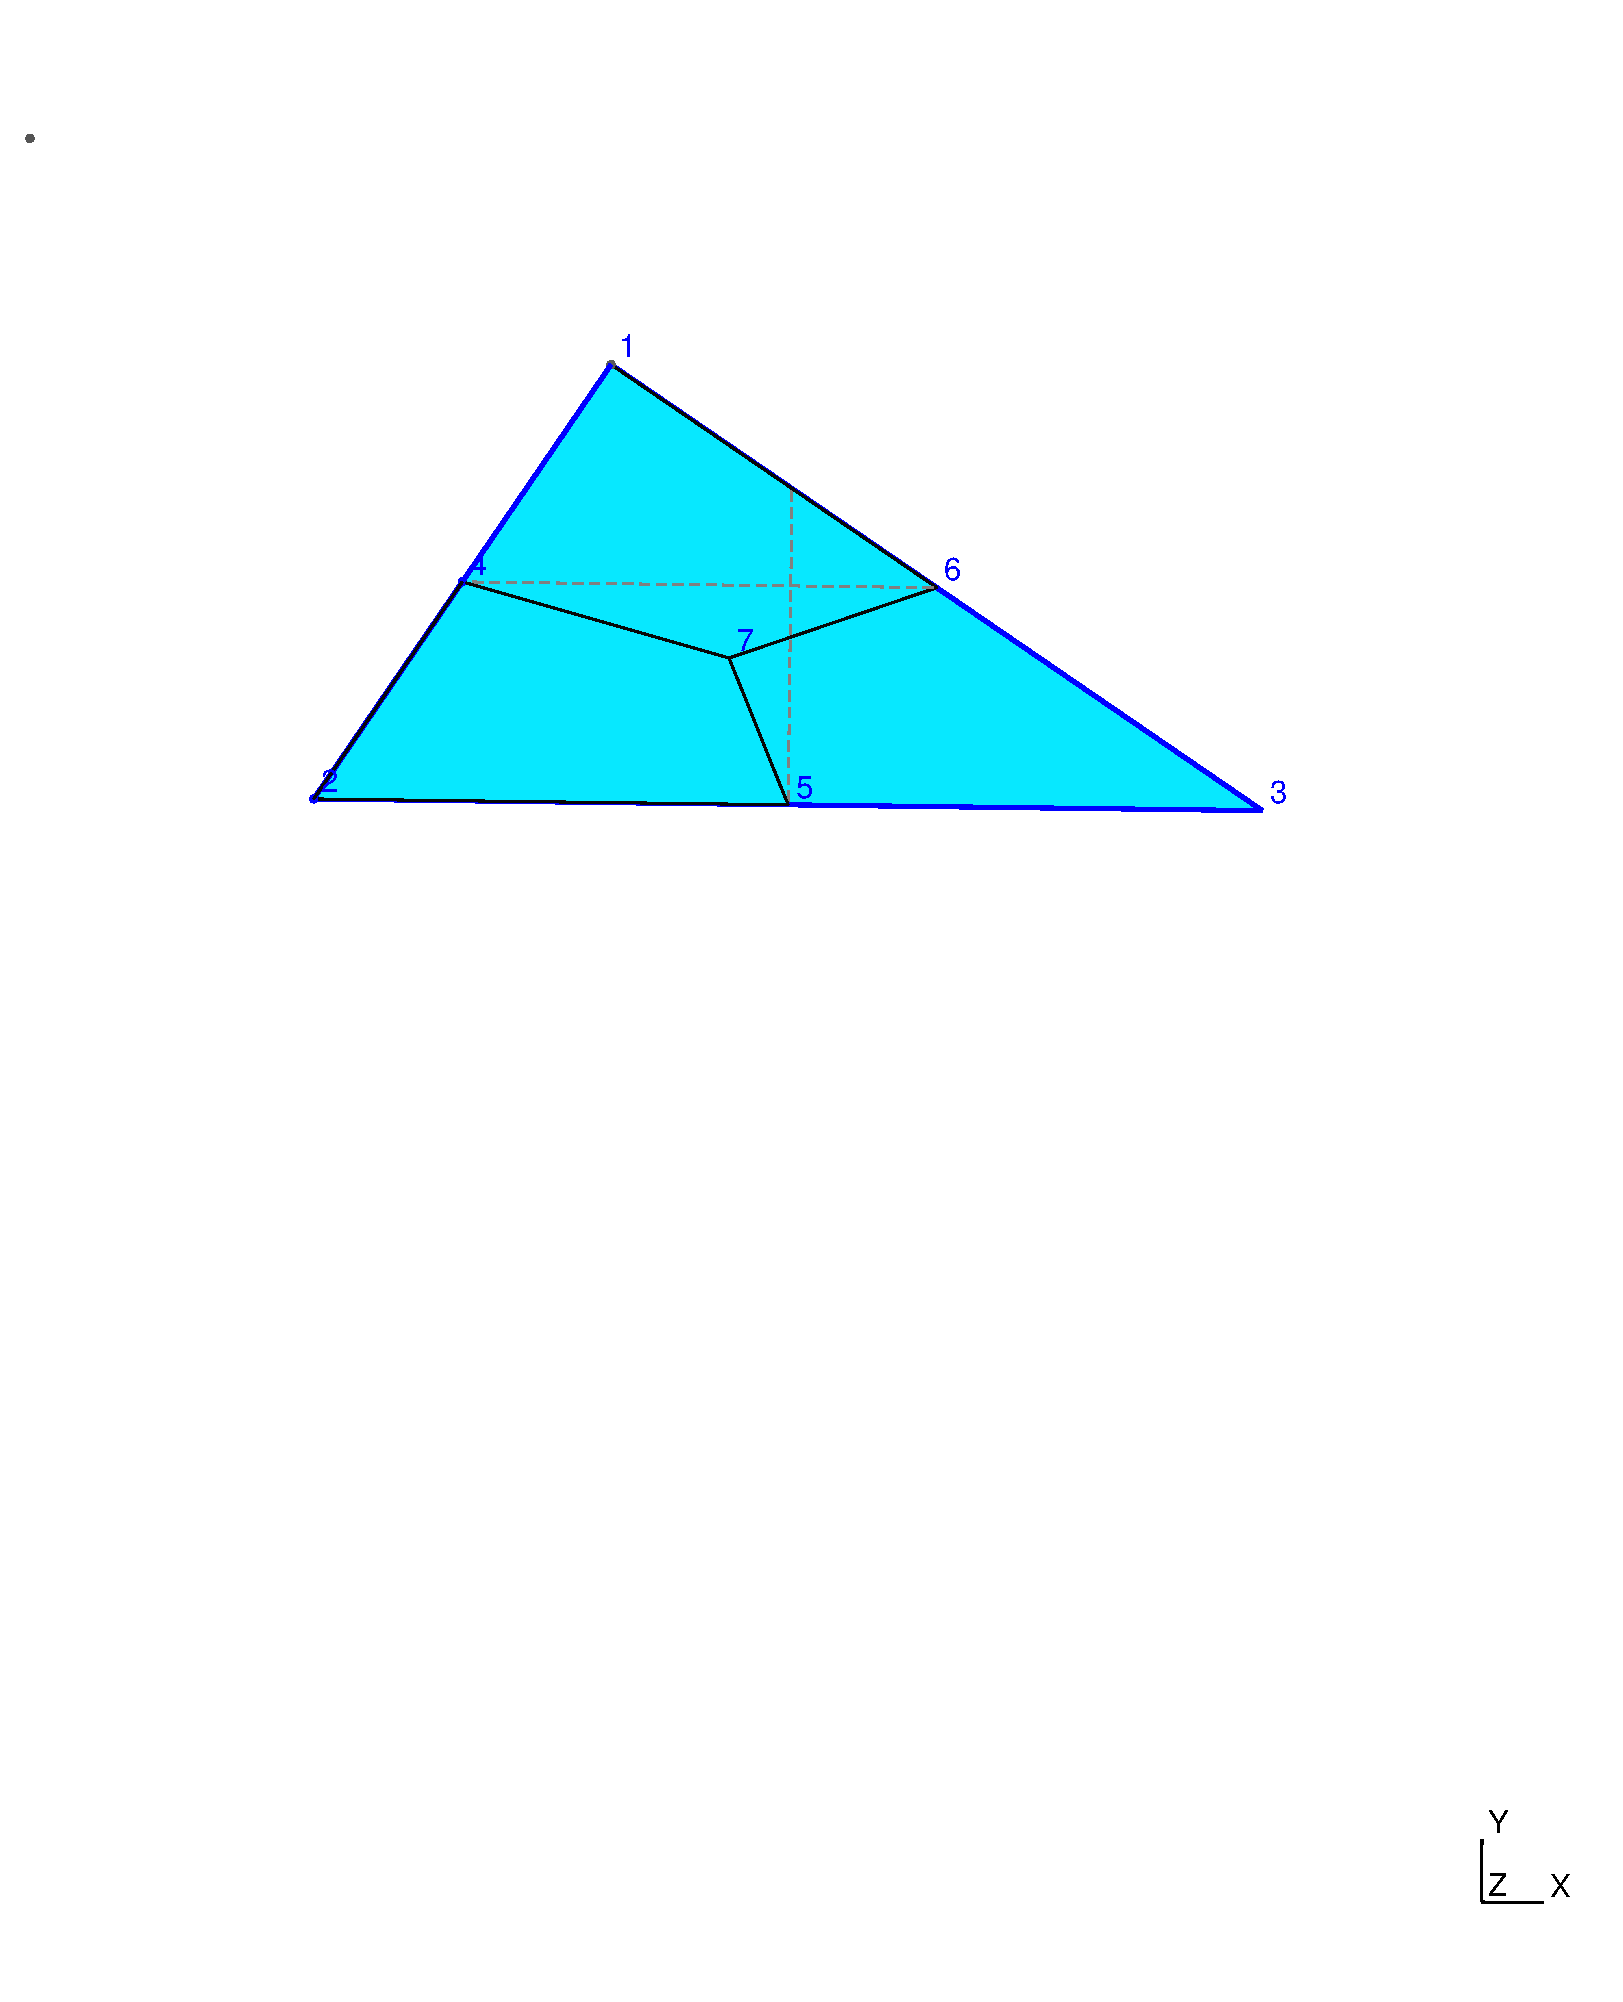
\includegraphics[trim = 0 550 0 100, clip,width=0.8\textwidth]{fig/meshgmsh.eps}
\caption{Mesh generated with gmsh.}
\end{figure}

\subsubsection{Module}

The mesh module contain a class that can be instantiate into a variable object. This mesh object has automatically intrinsic properties (because of the init method). Those properties are: the coordinates of the nodes arranged in a second order array with two columns and as many rows as the number of nodes; the connectivity matrix arranged in a second order array with 4 columns (quad elements) and as many rows as the number of elements. These properties corresponds to data attributes to the instance object mesh.

The mesh object also have method attributes ---\textsf{ Meshname.attribute() }--- which are functions that can be called with the intuitive namespace. For example, when computing each of the components of the matrix we call a method that computes the Jacobian for each element, individually, with the nodes that define the element as argument for each Gauss point.


\subsubsection{Methods}

\subsubsection*{basisFunction2D} which adds new attributes to the object. Those new attributes are: a first order array with the linear shape functions in 2-dimensions at a specific Gauss point.
\begin{equation*}
\textsf{mesh.phi} = \begin{bmatrix}
\phi^1(g_p, g_w) & \phi^2(g_p, g_w) & \phi^3(g_p, g_w) & \phi^4(g_p, g_w)
\end{bmatrix}^T
\end{equation*}
the second one is a second order array with the derivative of the shape functions with respect to the first and second natural coordinates (in the isoparametric domain).
\begin{equation*}
\textsf{mesh.dphi} = \begin{bmatrix}
\dfrac{\partial \phi^1}{\partial \xi_1} & \dfrac{\partial \phi^2}{\partial \xi_1} & \dfrac{\partial \phi^3}{\partial \xi_1} & \dfrac{\partial \phi^4}{\partial \xi_1}\\[.4cm]
\dfrac{\partial \phi^1}{\partial \xi_2} & \dfrac{\partial \phi^2}{\partial \xi_2} & \dfrac{\partial \phi^3}{\partial \xi_2} & \dfrac{\partial \phi^4}{\partial \xi_2}
\end{bmatrix}
\end{equation*}

\subsubsection*{mapping} changes the variable from the Cartesian coordinates into the natural domain, this is done by using
\begin{equation*}
x_i(\xi_I) = \sum_{k=1}^4 X^k_i \phi^k,
\end{equation*}
or,
\begin{equation*}
\begin{bmatrix}
x_1 \\[.2cm]
x_2
\end{bmatrix} = \begin{bmatrix}
X^1_1 \\[.2cm]
X^1_2
\end{bmatrix} \phi^1 +
\begin{bmatrix}
X^2_1 \\[.2cm]
X^2_2
\end{bmatrix} \phi^2 +
\begin{bmatrix}
X^3_1 \\[.2cm]
X^3_2
\end{bmatrix} \phi^3+
\begin{bmatrix}
X^4_1 \\[.2cm]
X^4_2
\end{bmatrix} \phi^4,
\end{equation*}
where, $X^k_i$ represent the $k$ node with coordinate $i$ of an individual element (with 4 nodes). The Cartesian coordinates will be a function of the natural coordinates, $x_i(\xi_I)$. The mapping is done so we can compute the integrals on the isoparametric domain using Gaussian Quadrature. This method is called when a integral is computed, inside a \textsf{for} loop.

\subsubsection*{eleJacobian}

This method creates a series of attributes related with the Jacobian matrix generated on the process of changing variables. It is called when a integral is calculated. The first attribute is the Jacobian matrix, expressed earlier. This matrix is obtained by the following multiplication,
\begin{equation*}
\mathsf{mesh.Jac} = 
\begin{bmatrix}
\dfrac{\partial \phi^1}{\partial \xi_1} & \dfrac{\partial \phi^2}{\partial \xi_1} & \dfrac{\partial \phi^3}{\partial \xi_1} & \dfrac{\partial \phi^4}{\partial \xi_1}\\[.4cm]
\dfrac{\partial \phi^1}{\partial \xi_2} & \dfrac{\partial \phi^2}{\partial \xi_2} & \dfrac{\partial \phi^3}{\partial \xi_2} & \dfrac{\partial \phi^4}{\partial \xi_2}
\end{bmatrix}
\begin{bmatrix}
X^1_1 & X^1_2 \\[.2cm]
X^2_1 & X^2_2 \\[.2cm]
X^3_1 & X^3_2 \\[.2cm]
X^4_1 & X^4_2 
\end{bmatrix},
\end{equation*} 
note that the Jacobian matrix is already in the natural coordinates. The next attribute is the determinant of this matrix, $\textsf{mesh.detJac}$. 

In order to use the chain rule we need the inverse of the Jacobian matrix, this is done by using a method from \textsf{NumPy} library.

The calculation of the entries of the stiffness matrix require the derivative of the shape functions with respect to the Cartesian coordinates. Because the coordinte system has changed, the derivative must be calculated with the chain rule. The attribute builds an 2x4 array with the gradient of each shape function, this is done by multiplying

\begin{equation*}
\textsf{mesh.dphi}\_\textsf{xi} = \begin{bmatrix}
\dfrac{\partial \xi_1}{\partial x_1} & \dfrac{\partial \xi_2}{\partial x_1} \\[.4cm]
\dfrac{\partial \xi_1}{\partial x_2} & \dfrac{\partial \xi_2}{\partial x_2}
\end{bmatrix}
\begin{bmatrix}
\dfrac{\partial \phi^1}{\partial \xi_1} & \dfrac{\partial \phi^2}{\partial \xi_1} & \dfrac{\partial \phi^3}{\partial \xi_1} & \dfrac{\partial \phi^4}{\partial \xi_1}\\[.4cm]
\dfrac{\partial \phi^1}{\partial \xi_2} & \dfrac{\partial \phi^2}{\partial \xi_2} & \dfrac{\partial \phi^3}{\partial \xi_2} & \dfrac{\partial \phi^4}{\partial \xi_2}
\end{bmatrix}
\end{equation*}

\subsubsection*{ArchLength}

This attributes to the object a vector with the 4 arch length for the change in coordinates on the line integral. From the Jacobian matrix,
\begin{equation*}
\textsf{mesh.Jac} = \begin{bmatrix}
\dfrac{\partial x_1}{\partial \xi_1} & \dfrac{\partial x_1}{\partial \xi_2}  \\[0.4cm]
\dfrac{\partial x_2}{\partial \xi_1} & \dfrac{\partial x_2}{\partial \xi_2} 
\end{bmatrix},
\end{equation*}
the arch length ratios are,
\begin{equation*}
\textsf{mesh.ArchLength} = \begin{bmatrix}
\sqrt{\textsf{mesh.Jac}[0,1]^2 + \textsf{mesh.Jac}[1,1]^2} \\[.3cm]
\sqrt{\textsf{mesh.Jac}[0,0]^2 + \textsf{mesh.Jac}[1,0]^2} \\[.3cm]
\sqrt{\textsf{mesh.Jac}[0,1]^2 + \textsf{mesh.Jac}[1,1]^2} \\[.3cm]
\sqrt{\textsf{mesh.Jac}[0,0]^2 + \textsf{mesh.Jac}[1,0]^2}
\end{bmatrix} = \begin{bmatrix}
\sqrt{\left(\dfrac{\partial x_1}{\partial \xi_2}\right)^2 + \left(\dfrac{\partial x_2}{\partial \xi_2}\right)^2}
 \\[.4cm]
\sqrt{\left(\dfrac{\partial x_1}{\partial \xi_1}\right)^2 + \left(\dfrac{\partial x_2}{\partial \xi_1}\right)^2} 
\\[.4cm]
\sqrt{\left(\dfrac{\partial x_1}{\partial \xi_2}\right)^2 + \left(\dfrac{\partial x_2}{\partial \xi_2}\right)^2} 
\\[.4cm]
\sqrt{\left(\dfrac{\partial x_1}{\partial \xi_1}\right)^2 + \left(\dfrac{\partial x_2}{\partial \xi_1}\right)^2}
\end{bmatrix}
\end{equation*}
The first entry is refereed to right side of the element with $\xi_1=1$, the second: top side with $\xi_2=1$, the third: left side with $\xi_1=-1$ and lastly the fourth: bottom side with $\xi_2=-1$.



\subsection{Gaussian Quadrature}





\subsection{Stiffness Matrix}

For each element the following integral must be solved in order to form the Elemental Stiffness Matrix which will be $8\; x\; 8$,
\begin{equation}
K_{ik}^{AB} = \int_{\Omega^e} \phi^A_{,j} \mathbb{C}_{ijk\ell} \;\phi^B_{,\ell}\; \mathrm{d} \Omega 
\end{equation}
So, the first thing we need is to deal with the fourth order elasticity tensor. This is done by using the fact that we are dealing with an isotropic material.

\subsubsection{Strain-Displacement in Matrix Form}

The strain-displacement (kinematics) in 2-dimension can be expressed as follows,
\begin{equation}
\begin{bmatrix}
\varepsilon_{11} \\
\varepsilon_{22} \\
\varepsilon_{12}
\end{bmatrix} 
= 
\begin{bmatrix}
\dfrac{\partial}{\partial x_1}  & 0 \\
0 &\dfrac{\partial}{\partial x_2} \\[0.4cm]
\dfrac{\partial}{\partial x_2}  &  \dfrac{\partial}{\partial x_1} 
\end{bmatrix}
\begin{bmatrix}
u_1 \\
u_2
\end{bmatrix}
=\mathbf{Du}
\end{equation}
where $\varepsilon_{12} = 2\gamma_{12} $ represents the engineering shear strain, this is useful because the matrix of partial derivatives is going to be convenient.

\subsubsection{Stress-Strain in Matrix Form}

Earlier, the strain was expressed using the stress. For two dimensions, 
\begin{align*}
\varepsilon_{11} &=  \dfrac{1}{E} \sigma_{11} - \frac{\nu}{E}\sigma_{22}\\
\varepsilon_{22} &= \dfrac{1}{E} \sigma_{22} - \frac{\nu}{E}\sigma_{11}\\
\varepsilon_{12} &= \dfrac{1 + \nu}{E} \sigma_{12} 
\end{align*}
relation that can be inverted to form the constitutive relation in matrix form,
\begin{equation}
\begin{bmatrix}
\sigma_{11} \\
\sigma_{22} \\
\sigma_{12}
\end{bmatrix}
=
\dfrac{E}{1- \nu^2}
\begin{bmatrix}
1 & \nu & 0 \\
\nu & 1 & 0 \\
0 & 0 & 1 - \nu
\end{bmatrix} 
\begin{bmatrix}
\varepsilon_{11} \\
\varepsilon_{22}\\
\varepsilon_{12}
\end{bmatrix}
=
\mathbf{C} \boldsymbol \varepsilon
\end{equation}

\subsubsection{Approximate Solution in Matrix Form}

The approximate solution, $\hat{u}_{_i}$, 
\begin{equation}
\hat{u}_i  =
\begin{bmatrix}
u^h_{1} \\[0.3cm]
u^h_{2}
\end{bmatrix}
=\sum_B^4
b^B_i \phi^B =
\begin{bmatrix}
 b^1_{1} \phi^1 + b^2_{1} \phi^2 + b^3_{1} \phi^3 + b^4_{1} \phi^4 \\[0.3cm]
 b^1_{2} \phi^1 + b^2_{2} \phi^2 + b^3_{2} \phi^3 + b^4_{2} \phi^4 
 \end{bmatrix}
\end{equation}
written in matrix form is,
\begin{equation}
\hat{u}_i =
\begin{bmatrix}
\phi^1  & 0 & \phi^2 & 0& \phi^3 & 0 & \phi^4 & 0\\
0 & \phi^1 & 0 &\phi^2  &0 & \phi^3 & 0 & \phi^4\\
\end{bmatrix}
\begin{bmatrix}
b^1_{1} \\[0.15cm]
b^1_{2} \\[0.15cm]
b^2_{1} \\[0.15cm]
b^2_{2} \\[0.15cm]
b^3_{1} \\[0.15cm]
b^3_{2} \\[0.15cm]
b^4_{1} \\[0.15cm]
b^4_{2} 
\end{bmatrix} = \boldsymbol \phi \mathbf{b}
\end{equation}
where, the constants $b^B_i$ are referent to each element.

\subsubsection{Shape Function's Gradient}

Substituting the approximate solution into the strain-displacement relations we will have to apply the derivative matrix, $\mathbf{D}$ into the shape functions, $\boldsymbol \phi$, forming,
\begin{equation}
\mathbf{D} = 
\begin{bmatrix}
\dfrac{\partial \phi^1}{\partial x_1}  & 0 & \dfrac{\partial \phi^2}{\partial x_1}  & 0 & \dfrac{\partial \phi^3}{\partial x_1}  & 0 & \dfrac{\partial \phi^4}{\partial x_1}  & 0\\[0.4cm]
0 & \dfrac{\partial \phi^1}{\partial x_2} & 0 & \dfrac{\partial \phi^2}{\partial x_2} & 0 & \dfrac{\partial \phi^3}{\partial x_2} & 0 & \dfrac{\partial \phi^4}{\partial x_2} \\[0.4cm]
\dfrac{\partial \phi^1}{\partial x_2} & \dfrac{\partial \phi^1}{\partial x_1} & \dfrac{\partial \phi^2}{\partial x_2} & \dfrac{\partial \phi^2}{\partial x_1} & \dfrac{\partial \phi^3}{\partial x_2} & \dfrac{\partial \phi^3}{\partial x_1} & \dfrac{\partial \phi^4}{\partial x_2} & \dfrac{\partial \phi^4}{\partial x_1} 
\end{bmatrix}
\end{equation}
using the isoparametric coordinate system and applying the chain rule, the matrix $\mathbf{D}$ becomes,
\begin{equation}
\mathbf{D} = \arraycolsep=3pt
\begin{bmatrix}
\dfrac{\partial \phi^1}{\partial \xi_I} \dfrac{\partial \xi_I}{\partial x_1}  & 0 & \dfrac{\partial \phi^2}{\partial \xi_I} \dfrac{\partial \xi_I}{\partial x_1}  & 0 & \dfrac{\partial \phi^3}{\partial \xi_I} \dfrac{\partial \xi_I}{\partial x_1}  & 0 & \dfrac{\partial \phi^4}{\partial \xi_I} \dfrac{\partial \xi_I}{\partial x_1}  & 0
\\[0.4cm]
0 & \dfrac{\partial \phi^1}{\partial \xi_I} \dfrac{\partial \xi_I}{\partial x_2} & 0 & \dfrac{\partial \phi^2}{\partial \xi_I} \dfrac{\partial \xi_I}{\partial x_2}  & 0 & \dfrac{\partial \phi^3}{\partial \xi_I} \dfrac{\partial \xi_I}{\partial x_2}  & 0 & \dfrac{\partial \phi^4}{\partial \xi_I} \dfrac{\partial \xi_I}{\partial x_2} 
\\[0.4cm]
\dfrac{\partial \phi^1}{\partial \xi_I} \dfrac{\partial \xi_I}{\partial x_2}  & \dfrac{\partial \phi^1}{\partial \xi_I} \dfrac{\partial \xi_I}{\partial x_1}  & \dfrac{\partial \phi^2}{\partial \xi_I} \dfrac{\partial \xi_I}{\partial x_2}  & \dfrac{\partial \phi^2}{\partial \xi_I} \dfrac{\partial \xi_I}{\partial x_1} & \dfrac{\partial \phi^3}{\partial \xi_I} \dfrac{\partial \xi_I}{\partial x_2}  & \dfrac{\partial \phi^3}{\partial \xi_I} \dfrac{\partial \xi_I}{\partial x_1}  & \dfrac{\partial \phi^4}{\partial \xi_I} \dfrac{\partial \xi_I}{\partial x_2}  & \dfrac{\partial \phi^4}{\partial \xi_I} \dfrac{\partial \xi_I}{\partial x_1} 
\end{bmatrix}
\end{equation}
each derivative has a summation implied with the $I$ index, this comes from the chain rule.

\subsubsection{Build}

In order to build the stiffness matrix, we need first evaluate the functions at the GP and then do the matrix multiplication. This is done by looping over each element and building from within this specific element its Jacobian matrix and anything else it might need, then, build the Elemental Stiffness matrix.
\begin{equation}
\mathbf{K^e} = \mathbf{D}^T \mathbf{C} \mathbf{D} \det[\mathbf{J}]
\end{equation}
So, the matrix $\mathbf{C}$ is $3 \; x\;3$ times the matrix $\mathbf{D}$ which is $3\;x\;8$ results in a $3\;x\;8$. Multiplying a $8\;x\;3$ by a $3\;x\;8$ results in a $8\;x\;8$  stiffness matrix.



\subsection{Load Vector}

For each element the following integral must be solved for each one of the 4 shape functions.
\begin{equation}
F_i^A = \int_{\Omega^e_\xi} \phi^A(\xi_I) f_i(\xi_I) \det[x_{i,I}] \; \mathrm{d} \Omega.
\end{equation}
Then, inside a loop for each element there is another loop with 4 steps that consider each of the 4 different GP in order to evaluate all the functions at those points. Next, compute the Jacobian based on the specific element nodes coordinates. After that we will need the mapping for $x_1 (\xi_I)$ and $x_2 (\xi_I)$ in order to compute the elemental load in the isoparametric domain. Therefore, for each GP we will have the following matrix product.
\begin{equation}
\mathbf{F} = \boldsymbol \phi^T \mathbf{f} \det[\mathbf{J}]
\end{equation}




\subsection{Traction Vector}

The traction vector is calculated from the integral for each element,
\begin{equation}
T_i^L = \int_{\Gamma} \; \phi^L(\xi_I) \bar{t}_i(\xi_I) \det[J_s]\; \mathrm{d} S,
\end{equation}
because we are diving the domain boundary into 4 different paths, then we have,
\begin{multline*}
T_i^A=
\int_{\Gamma^1} \phi^A(1, \xi_2) \; \bar{t}_i(1, \xi_2) \sqrt{\left(\dfrac{\partial x_1}{\partial \xi_2}\right)^2 + \left(\dfrac{\partial x_2}{\partial \xi_2}\right)^2}\, \mathrm{d} \xi_2 
+ \\
\int_{\Gamma^2} \phi^A(\xi_1, 1) \; \bar{t}_i(\xi_1, 1) \sqrt{\left(\dfrac{\partial x_1}{\partial \xi_1}\right)^2 + \left(\dfrac{\partial x_2}{\partial \xi_1}\right)^2}\, \mathrm{d} \xi_1
+ \\
\int_{\Gamma^3} \phi^A(1, \xi_2)\;  \bar{t}_i(1, \xi_2) \sqrt{\left(\dfrac{\partial x_1}{\partial \xi_2}\right)^2 + \left(\dfrac{\partial x_2}{\partial \xi_2}\right)^2}\, \mathrm{d} \xi_2 
+ \\
\int_{\Gamma^4} \phi^A(\xi_1, 1) \; \bar{t}_i(\xi_1, 1) \sqrt{\left(\dfrac{\partial x_1}{\partial \xi_1}\right)^2 + \left(\dfrac{\partial x_2}{\partial \xi_1}\right)^2}\, \mathrm{d} \xi_1
\end{multline*}
however, when specifying the traction boundary condition at a specific boundary, the boundary elements should have a tag identifying them according to the BC. At the end we should have a list of elements and all sides where the boundary is applied. Then we only have to compute the integral referent to those specific sides $L$, each element can have from 1 to 4 sides, $S^t$, with traction  to them. So, we can rewrite the traction integral,
\begin{equation}
T_i^A= \sum_{L=1}^{S^t}
\int_{\Gamma^L} \phi^A(\xi^L) \; \bar{t}_i(\xi^L) J_s^L\, \mathrm{d} S^L,
\end{equation}
where, $\Gamma^L$ is the side with traction, $\xi^L$ is the coordinate that defines a path $L$, $J^L_s$ is the jacobian for line integral referent to the path $L$ and $\mathrm{d} S^L$ is the differential referent to the path $L$. 

The next step is to compute the integral using Gaussian Quadrature, this case we will have two GP. Then, for each path we will have a summation of two GP. This can be view in matrix form as,
\begin{equation}
\mathbf{T} = \sum_{L=1}^{S^t} \boldsymbol \phi^T  \mathbf{\bar{t}}  \det[\mathbf{J_s^L}]
\end{equation}

\section{Results for Displacement Field}




\section{Stress Recovery}

Stress recovery is the procedure to compute the stress field from the fem solution.

\subsection{From Displacements}

In order to obtain the stress from the displacements calculated we need to compute the strain field and use the constituve relation. The strains are calculated from the expression:
\begin{equation}
\begin{bmatrix}
\varepsilon_{11} \\
\varepsilon_{22} \\
\varepsilon_{12}
\end{bmatrix} 
= 
\begin{bmatrix}
\dfrac{\partial}{\partial x_1}  & 0 \\
0 &\dfrac{\partial}{\partial x_2} \\[0.4cm]
\dfrac{\partial}{\partial x_2}  &  \dfrac{\partial}{\partial x_1} 
\end{bmatrix}
\begin{bmatrix}
u_1 \\
u_2
\end{bmatrix}
=\mathbf{Du}.
\end{equation}
The derivative of the displacements are computed using the approximated solution,
\begin{equation}
\begin{bmatrix}
\varepsilon_{11}\\
\varepsilon_{22}\\
\varepsilon_{12}
\end{bmatrix} 
=
\begin{bmatrix}
\dfrac{\partial}{\partial x_1}  & 0 \\
0 &\dfrac{\partial}{\partial x_2} \\[0.4cm]
\dfrac{\partial}{\partial x_2}  &  \dfrac{\partial}{\partial x_1} 
\end{bmatrix}
\begin{bmatrix}
b_1^1 \phi^1 + b_1^2 \phi^2 + b_1^3 \phi^3 + b^4_1 \phi^4 \\
b_2^1 \phi^1 + b_2^2 \phi^2 + b_2^3 \phi^3 + b^4_2 \phi^4
\end{bmatrix}.
\end{equation}

\begin{figure}[H]
\centering
	\begin{subfigure}[H]{0.49\textwidth}
		\includegraphics[width=\textwidth]{fig/ex1_elements.eps}
		\caption{}
		\label{fig:1}
	\end{subfigure}
	\begin{subfigure}[H]{0.49\textwidth}
		\includegraphics[width=\textwidth]{fig/ex1_deformation.eps}
		\caption{}
		\label{fig:2}
	\end{subfigure}	
	\begin{subfigure}[H]{0.49\textwidth}
		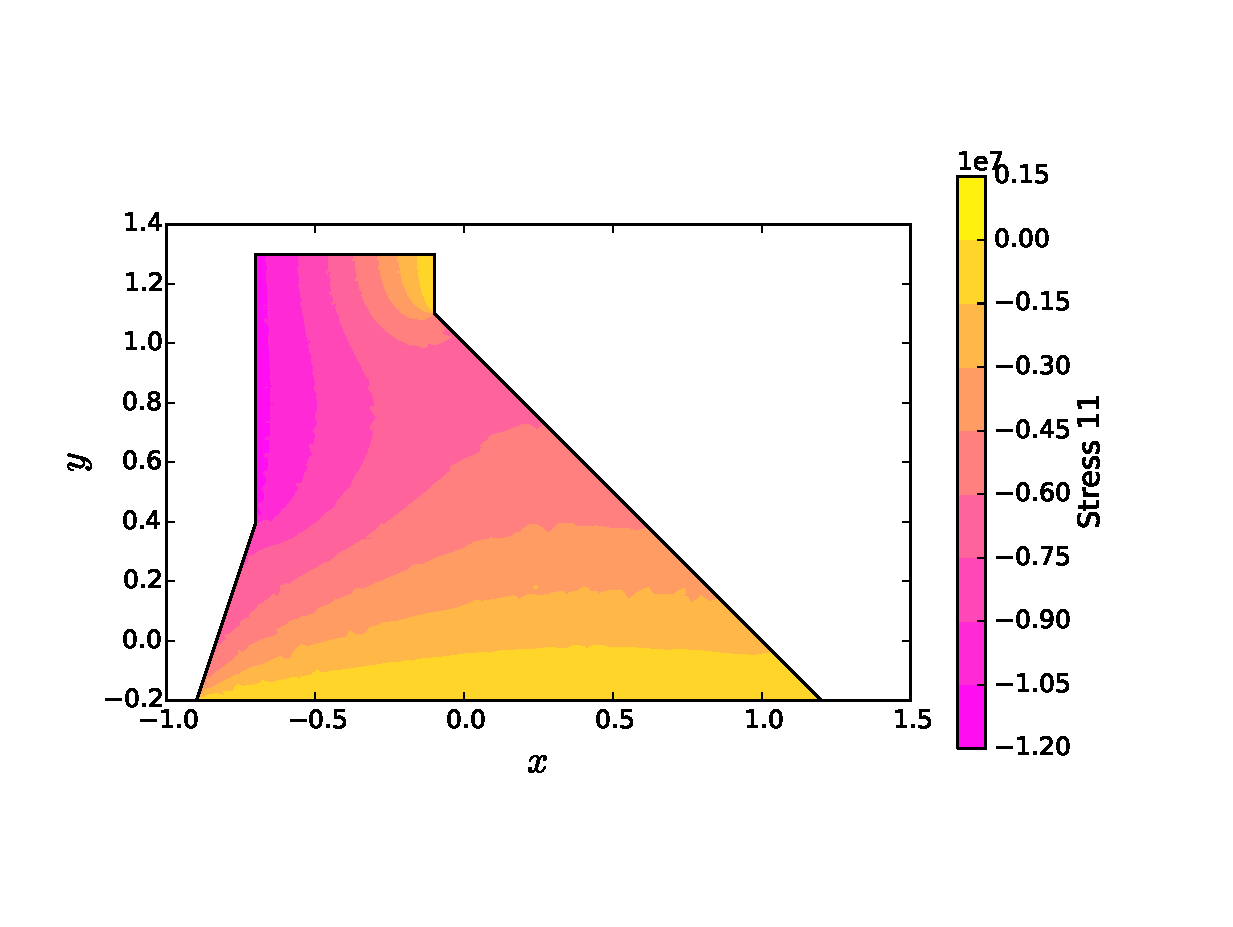
\includegraphics[width=1.2\textwidth]{fig/ex1_stress_11.eps}
		\caption{}
		\label{fig:1}
	\end{subfigure}
	\begin{subfigure}[H]{0.49\textwidth}
		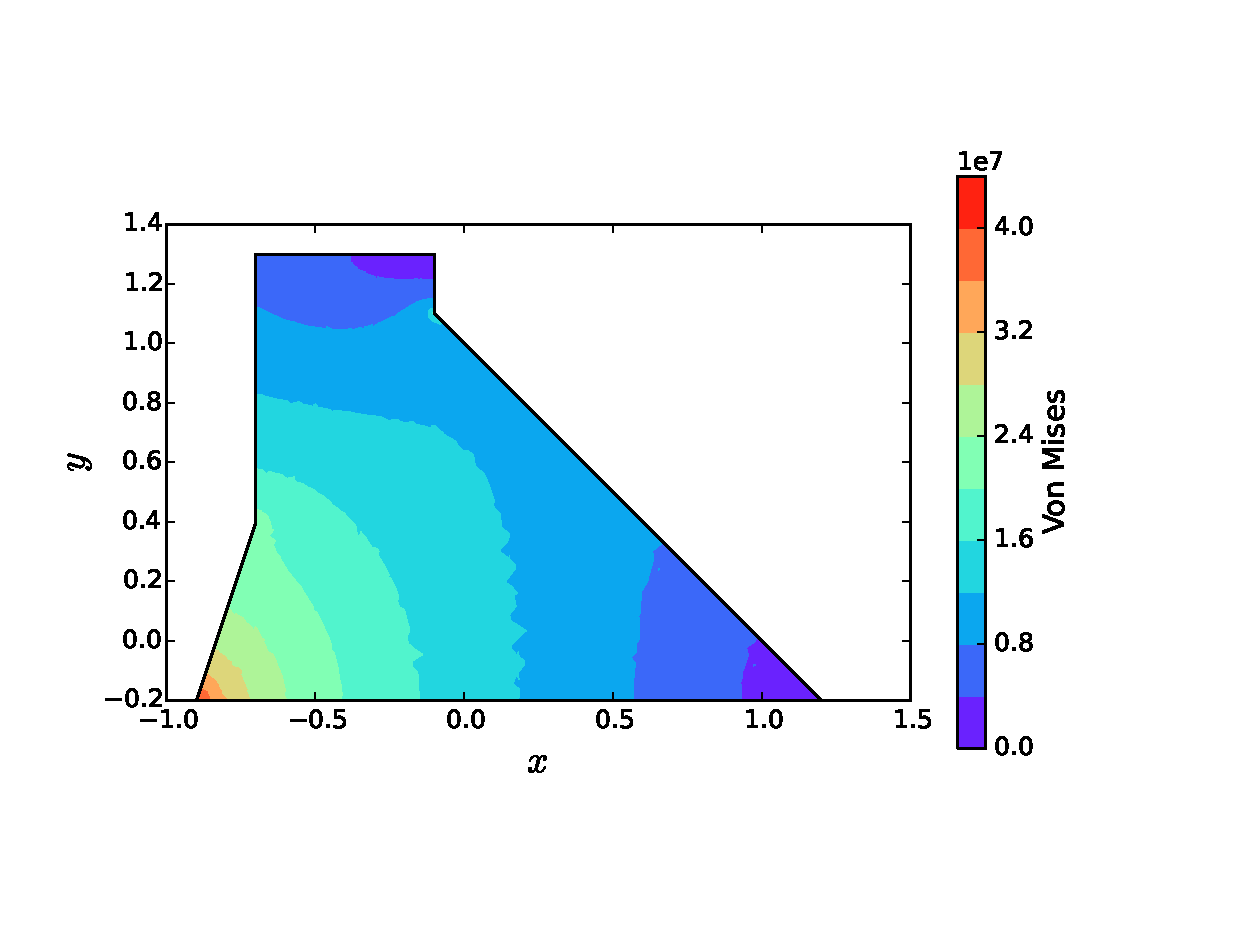
\includegraphics[width=1.2\textwidth]{fig/ex1_von_mises.eps}
		\caption{}
		\label{fig:2}
	\end{subfigure}
	\caption{Fig(a) shows the mesh used. Fig(b) the deformation of the structure after applying a force on the boundary line 0 and 1 of $5 \cdot 10^{-2}$ with $E=200 \cdot 10^{-2}$ and $\nu=0.3$ and the bottom, boundary line 2, is fixed. Fig(c) shows the normal stress on the x direction and Fig(d) shows the Von-Mises stress.}
	\label{fig:3_1}
\end{figure}


\subsection{48 Elements}

\begin{figure}[H]
\centering
	\begin{subfigure}[H]{0.49\textwidth}
		\includegraphics[width=\textwidth]{fig/ex2_elements.eps}
		\caption{}
		\label{fig:1}
	\end{subfigure}
	\begin{subfigure}[H]{0.49\textwidth}
		\includegraphics[width=\textwidth]{fig/ex2_deformation.eps}
		\caption{}
		\label{fig:2}
	\end{subfigure}	
	\begin{subfigure}[H]{0.49\textwidth}
		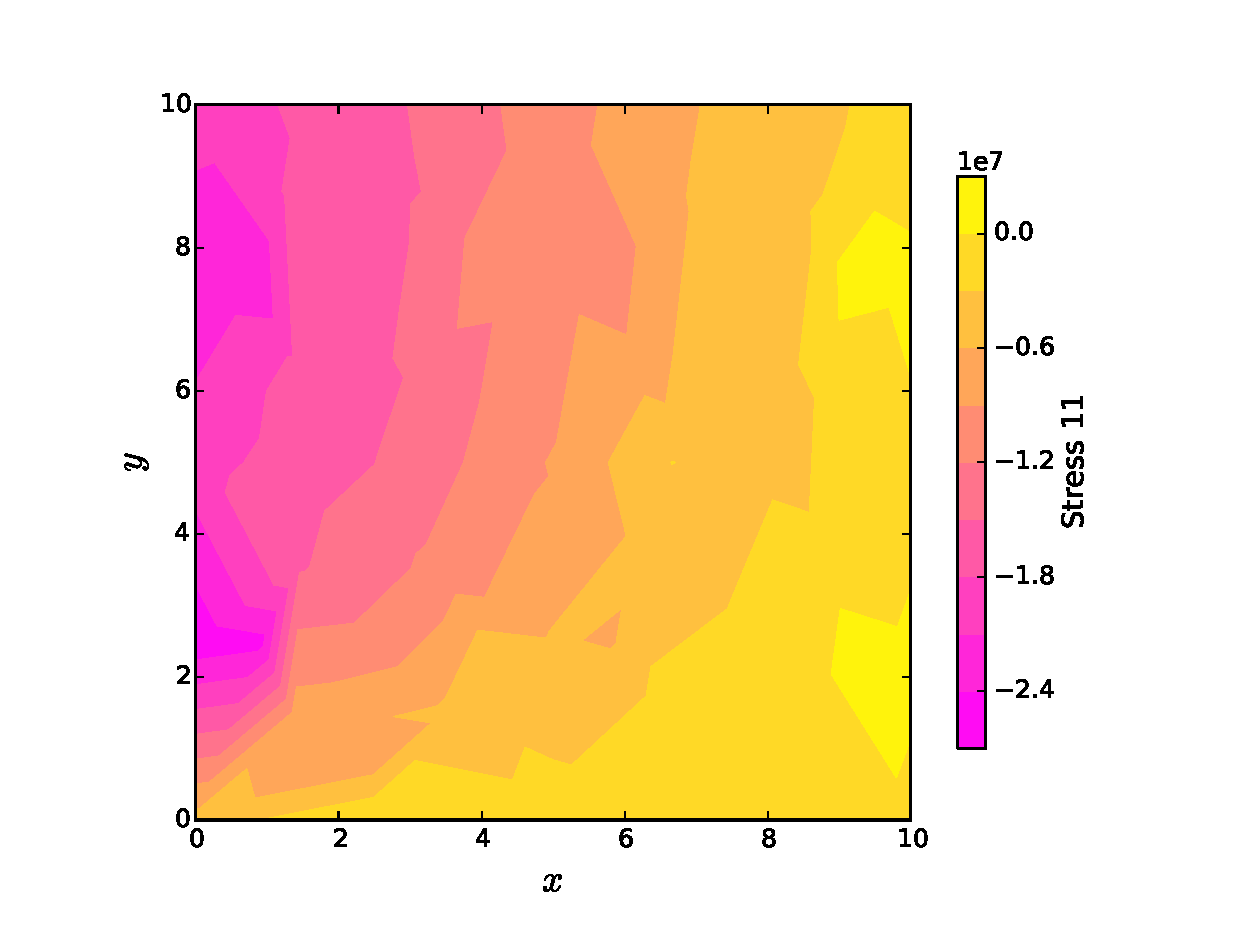
\includegraphics[width=\textwidth]{fig/ex2_stress_11.eps}
		\caption{}
		\label{fig:1}
	\end{subfigure}
		\begin{subfigure}[H]{0.49\textwidth}
		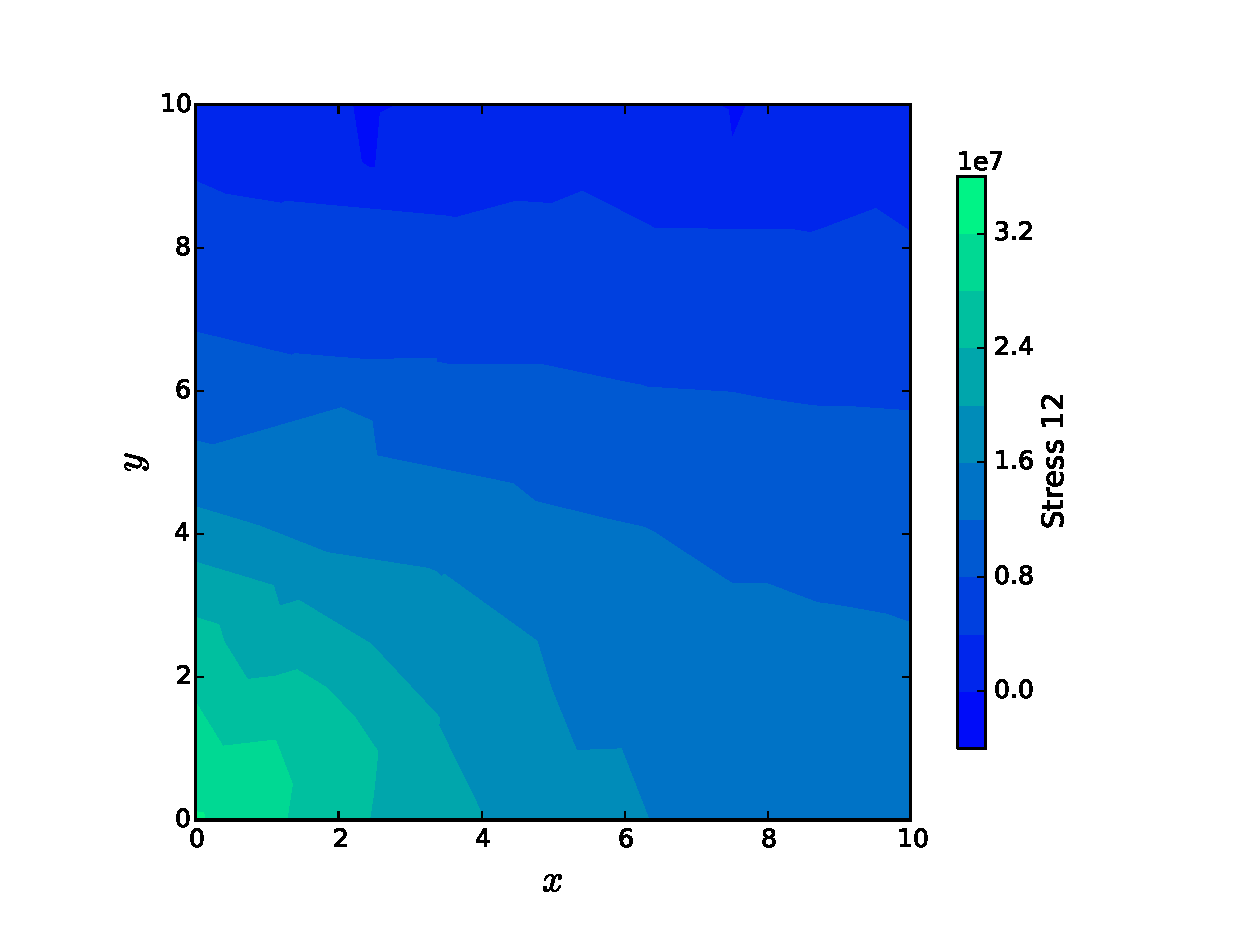
\includegraphics[width=\textwidth]{fig/ex2_stress_12.eps}
		\caption{}
		\label{fig:1}
	\end{subfigure}
	\begin{subfigure}[H]{0.49\textwidth}
		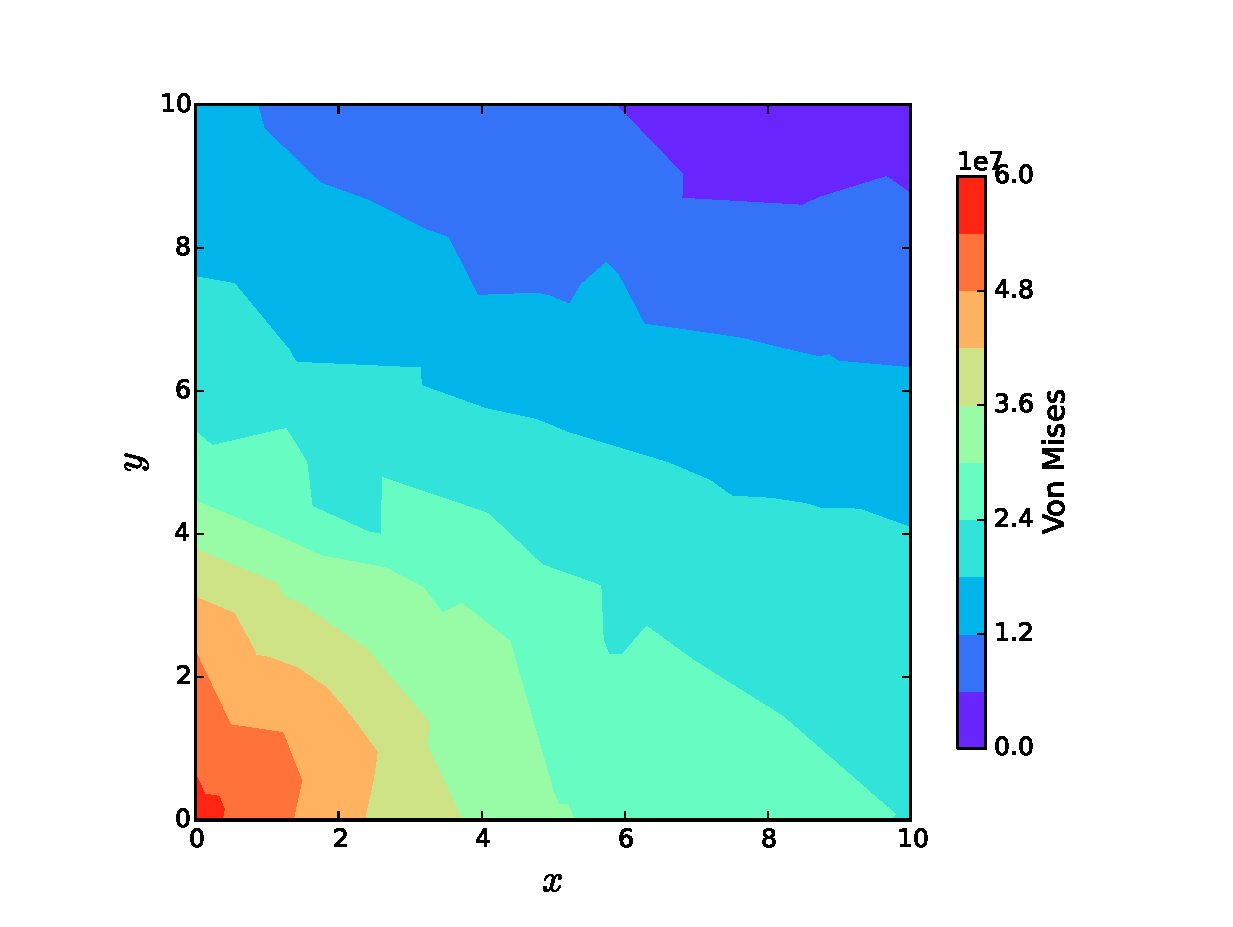
\includegraphics[width=\textwidth]{fig/ex2_von_mises.eps}
		\caption{}
		\label{fig:2}
	\end{subfigure}
	\begin{subfigure}[H]{0.49\textwidth}
		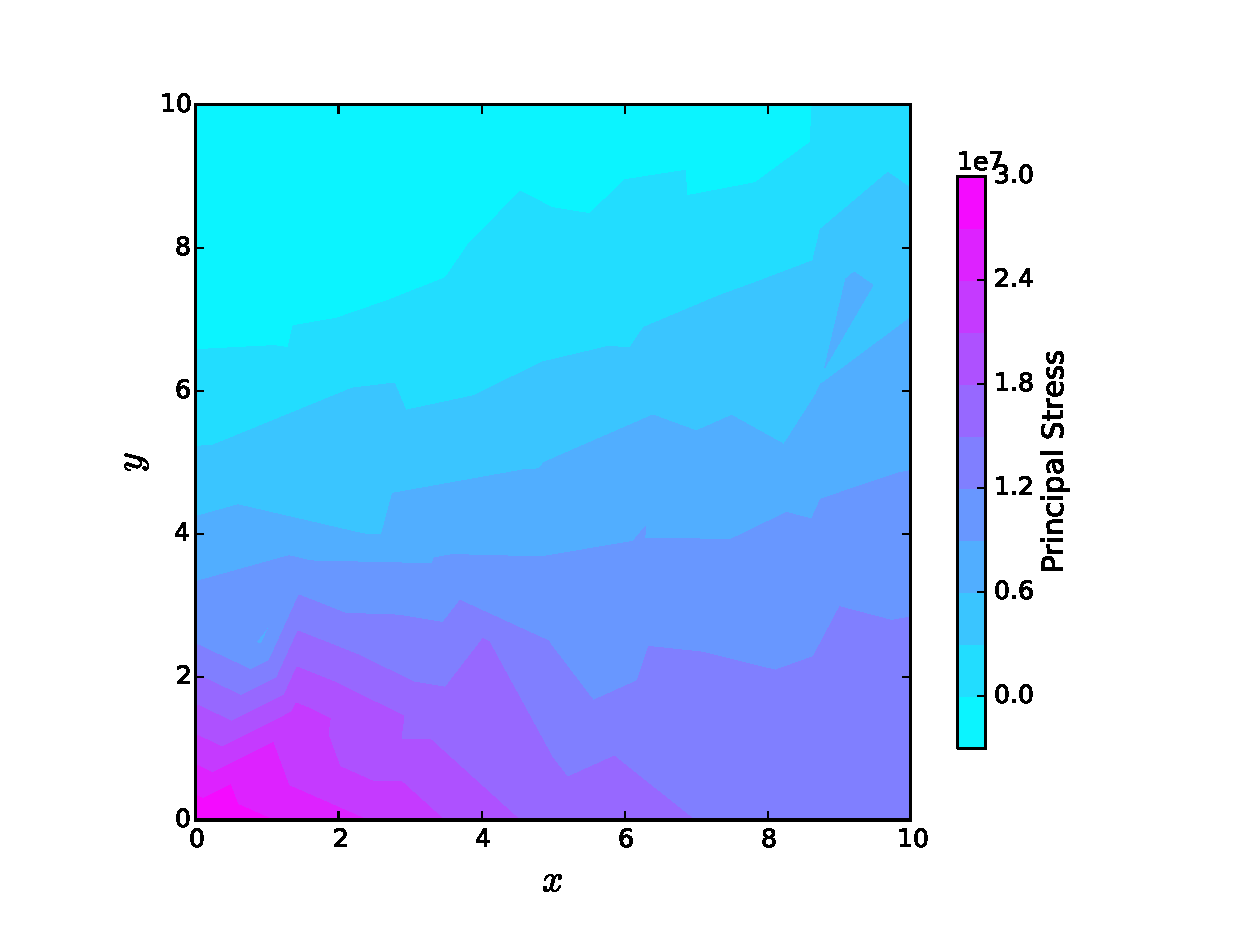
\includegraphics[width=\textwidth]{fig/ex2_principal_stress.eps}
		\caption{}
		\label{fig:2}
	\end{subfigure}
	\caption{Fig(a) shows the mesh used. Fig(b) the deformation of the structure after applying a force of $[0.1, 0]$ on the boundary line 3 with $E=200 \cdot 10^{-2}$ and $\nu=0.3$ and the bottom, boundary line 0, is fixed. Fig(c) shows the normal stress on the x direction, Fig(d) shows the shear stress, Fig(e) Von Mises stress and Fig(f) principal stress. Number of Elements: 48}
	\label{fig:3_1}
\end{figure}

\subsection{2028 Elements}


\begin{figure}[H]
\centering
	\begin{subfigure}[H]{0.49\textwidth}
		\includegraphics[width=\textwidth]{fig/ex3_elements.eps}
		\caption{}
		\label{fig:1}
	\end{subfigure}
	\begin{subfigure}[H]{0.49\textwidth}
		\includegraphics[width=\textwidth]{fig/ex3_deformation.eps}
		\caption{}
		\label{fig:2}
	\end{subfigure}	
	\begin{subfigure}[H]{0.49\textwidth}
		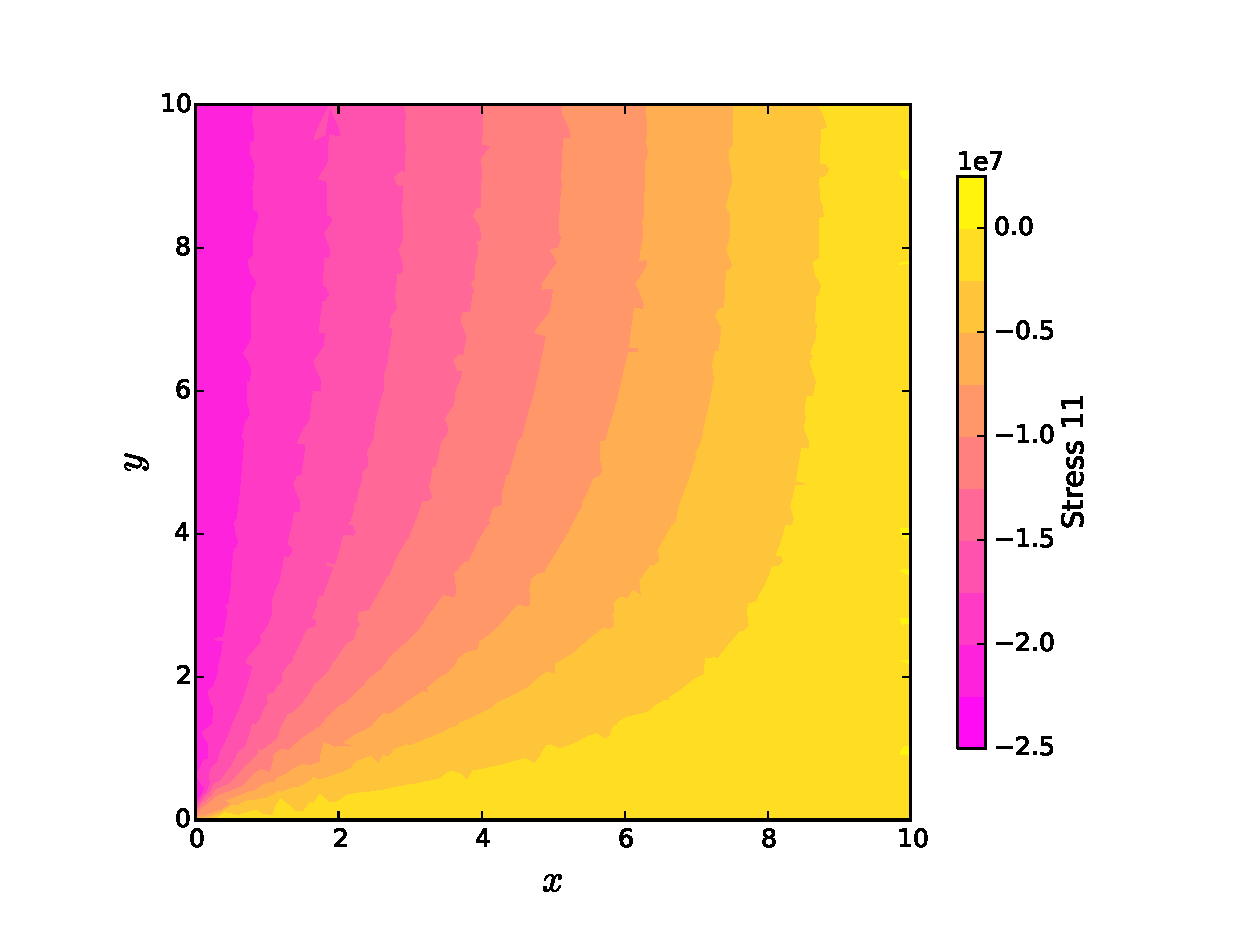
\includegraphics[width=\textwidth]{fig/ex3_stress_11.eps}
		\caption{}
		\label{fig:1}
	\end{subfigure}
		\begin{subfigure}[H]{0.49\textwidth}
		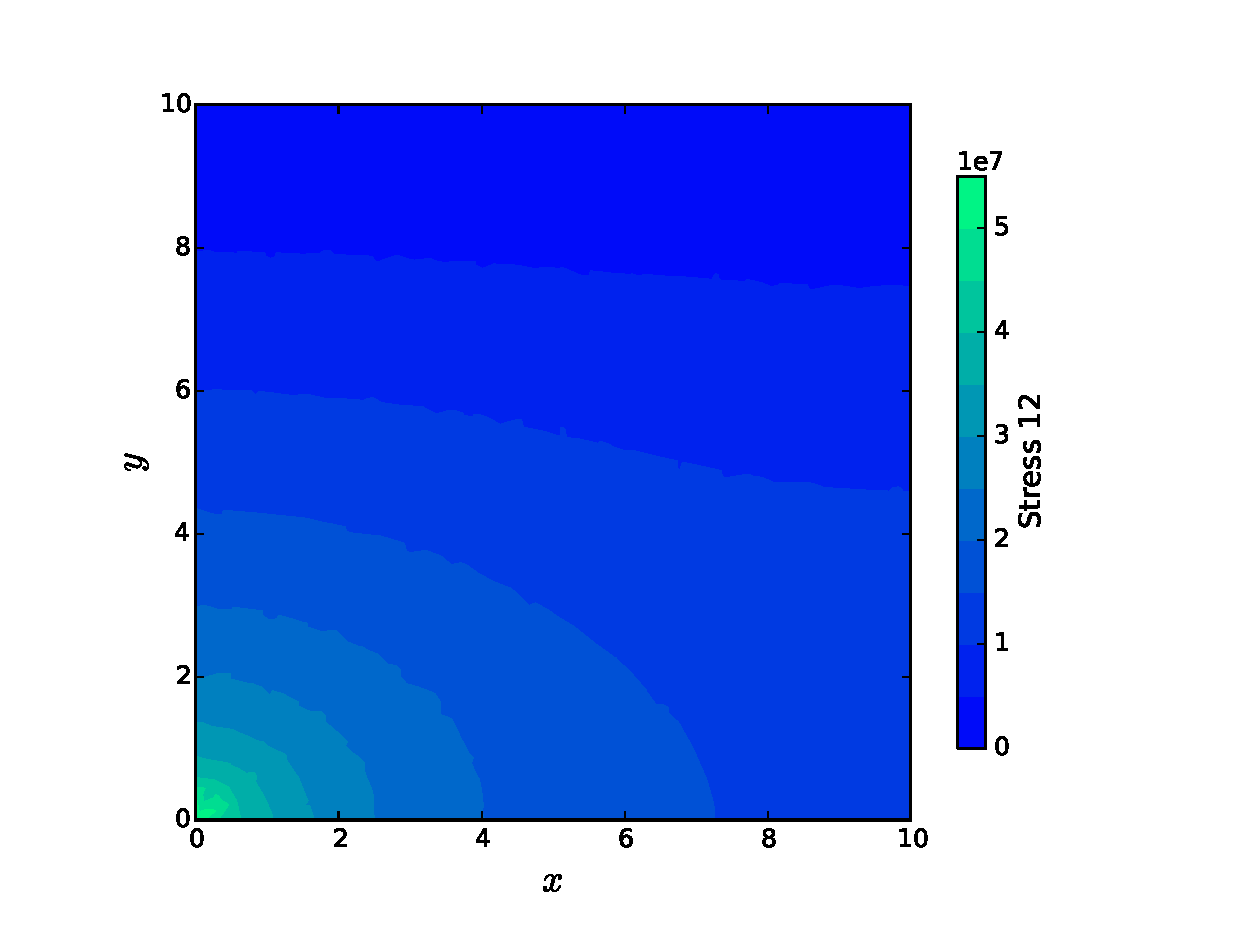
\includegraphics[width=\textwidth]{fig/ex3_stress_12.eps}
		\caption{}
		\label{fig:1}
	\end{subfigure}
	\begin{subfigure}[H]{0.49\textwidth}
		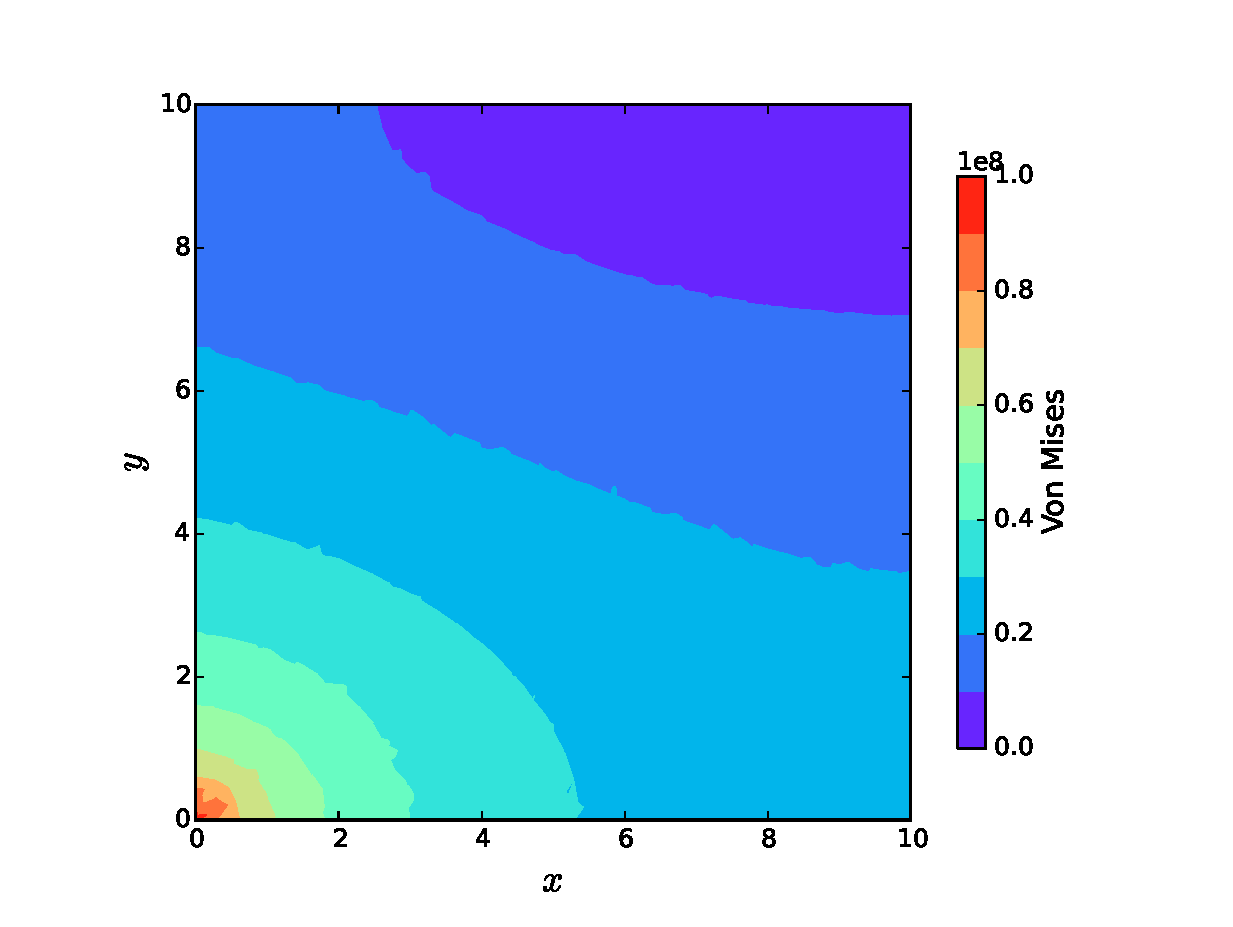
\includegraphics[width=\textwidth]{fig/ex3_von_mises.eps}
		\caption{}
		\label{fig:2}
	\end{subfigure}
	\begin{subfigure}[H]{0.49\textwidth}
		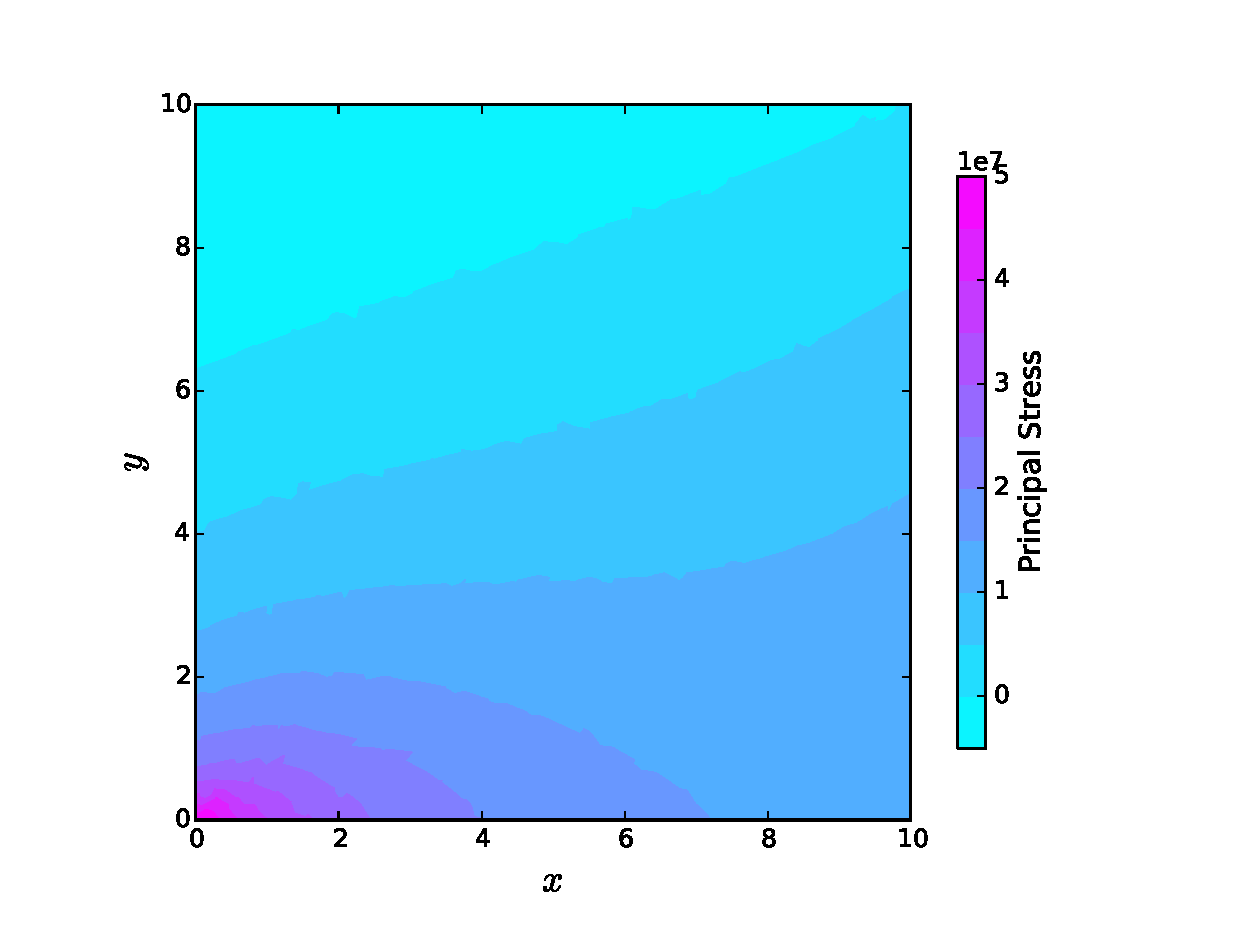
\includegraphics[width=\textwidth]{fig/ex3_principal_stress.eps}
		\caption{}
		\label{fig:2}
	\end{subfigure}
	\caption{Fig(a) shows the mesh used. Fig(b) the deformation of the structure after applying a force of $[0.1, 0]$ on the boundary line 3 with $E=200 \cdot 10^{-2}$ and $\nu=0.3$ and the bottom, boundary line 0, is fixed. Fig(c) shows the normal stress on the x direction, Fig(d) shows the shear stress, Fig(e) Von Mises stress and Fig(f) principal stress. Number of Elements: 2028}
	\label{fig:3_1}
\end{figure}


\subsection{2028 Elements - Interpolation from Gauss Points}


\begin{figure}[H]
\centering
	\begin{subfigure}[H]{0.49\textwidth}
		\includegraphics[width=\textwidth]{fig/ex4_elements.eps}
		\caption{}
		\label{fig:1}
	\end{subfigure}
	\begin{subfigure}[H]{0.49\textwidth}
		\includegraphics[width=\textwidth]{fig/ex4_deformation.eps}
		\caption{}
		\label{fig:2}
	\end{subfigure}	
	\begin{subfigure}[H]{0.49\textwidth}
		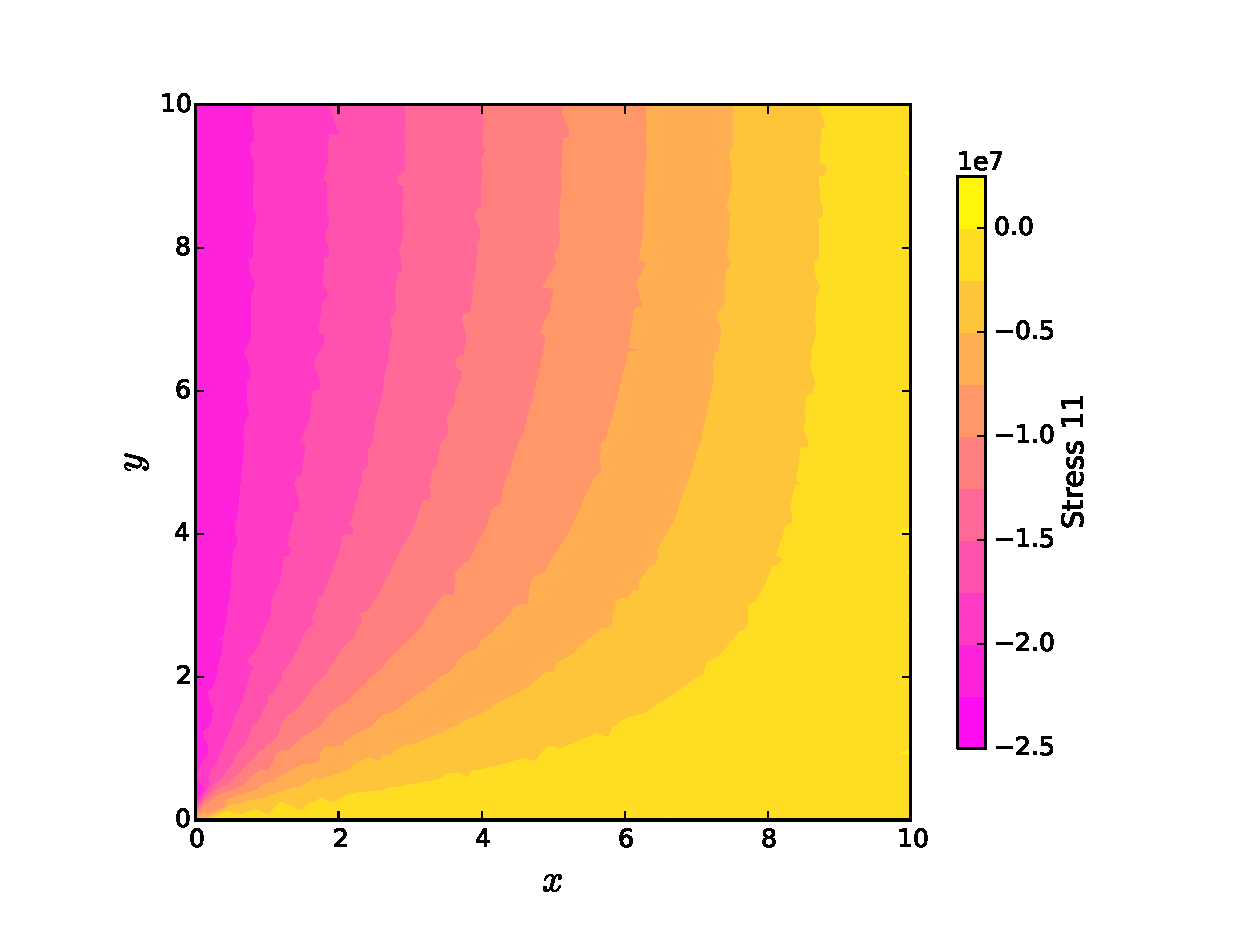
\includegraphics[width=\textwidth]{fig/ex4_stress_11.eps}
		\caption{}
		\label{fig:1}
	\end{subfigure}
		\begin{subfigure}[H]{0.49\textwidth}
		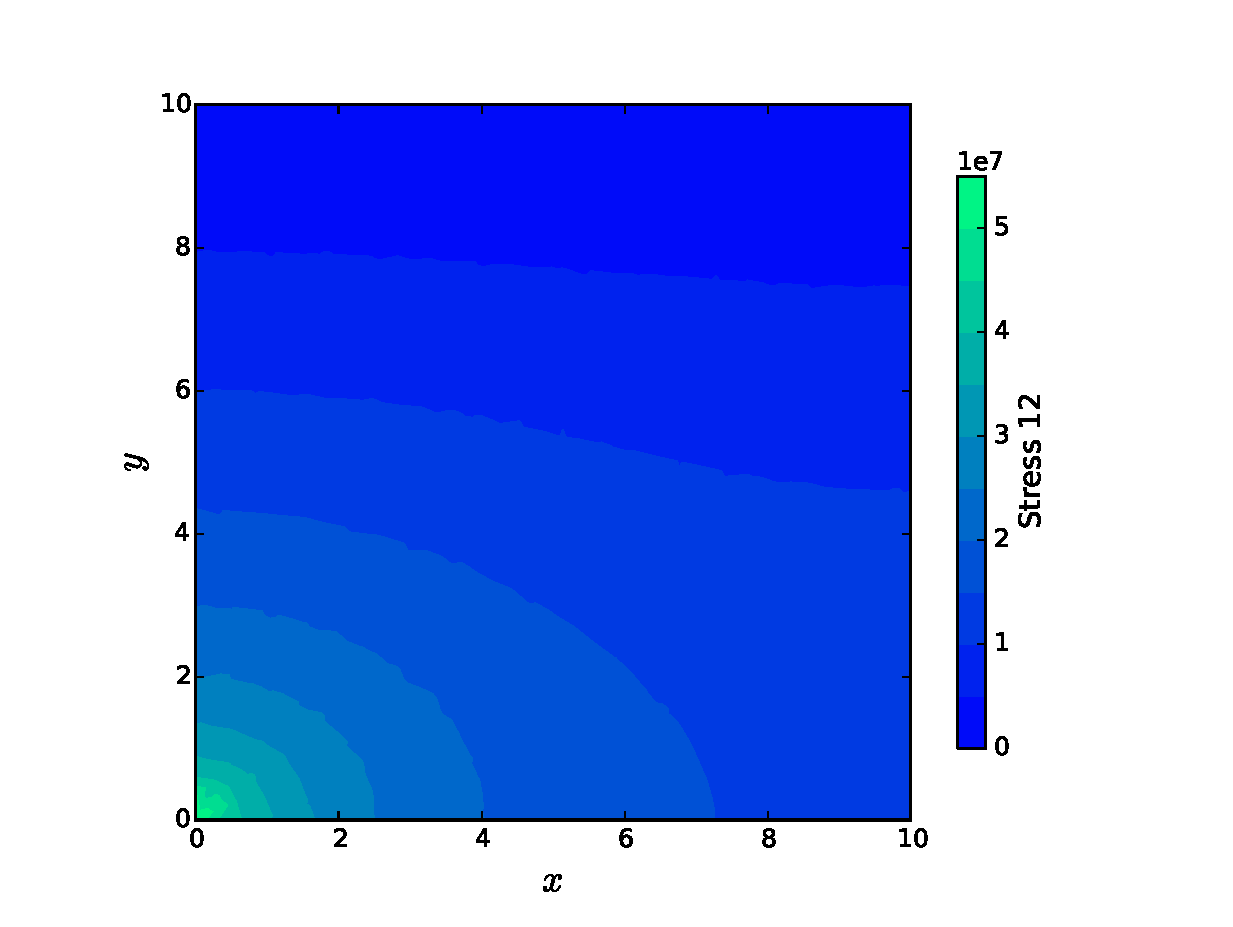
\includegraphics[width=\textwidth]{fig/ex4_stress_12.eps}
		\caption{}
		\label{fig:1}
	\end{subfigure}
	\begin{subfigure}[H]{0.49\textwidth}
		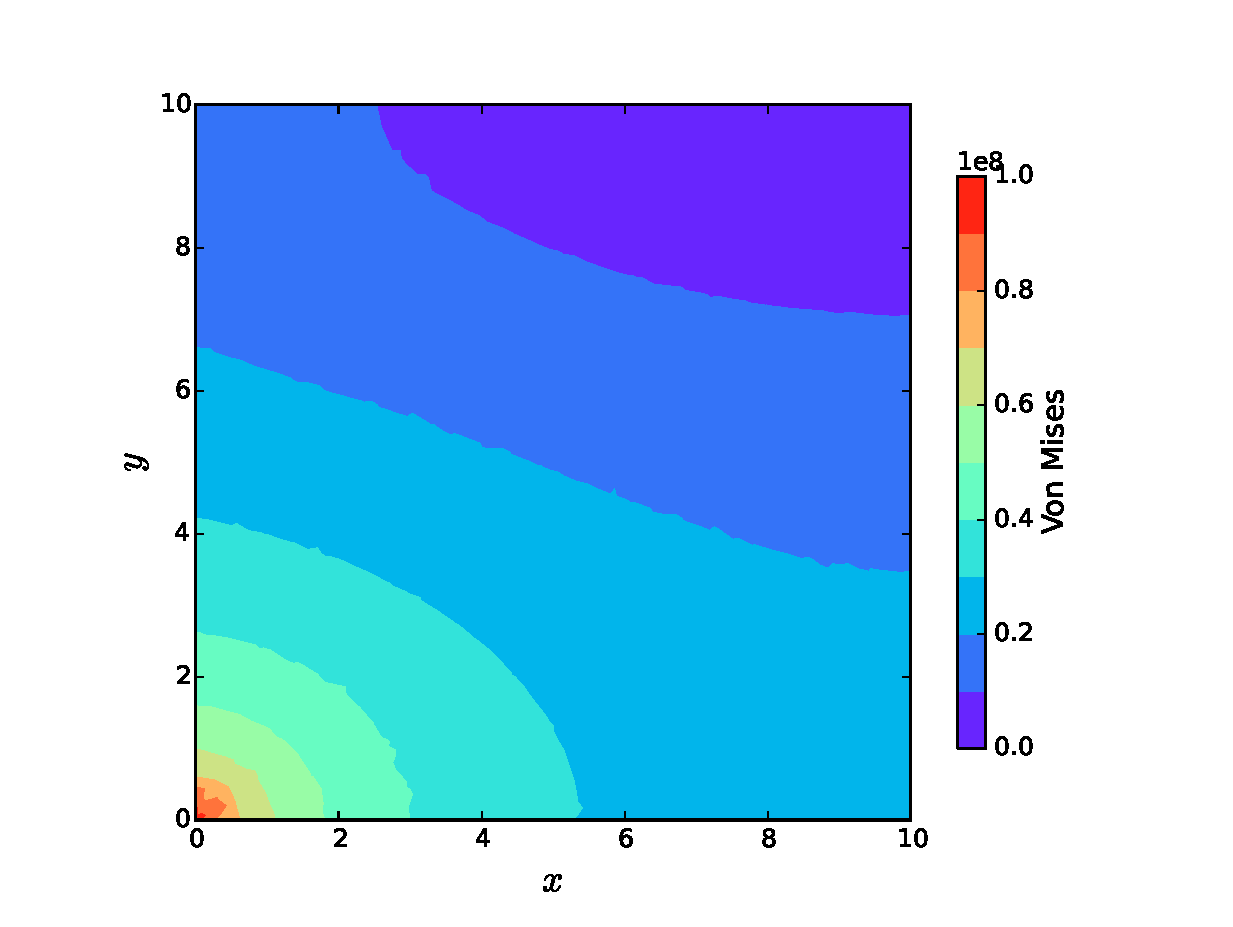
\includegraphics[width=\textwidth]{fig/ex4_von_mises.eps}
		\caption{}
		\label{fig:2}
	\end{subfigure}
	\begin{subfigure}[H]{0.49\textwidth}
		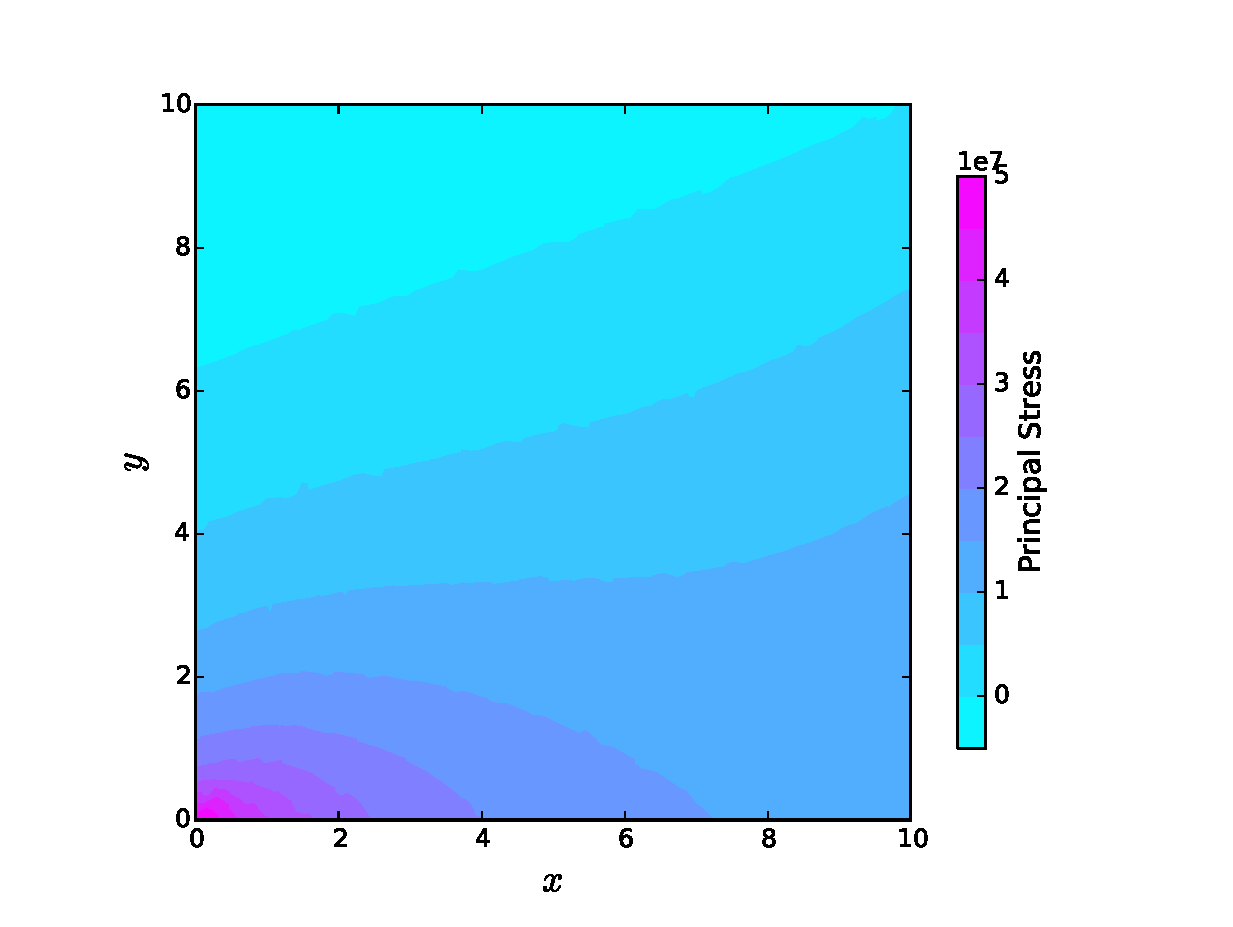
\includegraphics[width=\textwidth]{fig/ex4_principal_stress.eps}
		\caption{}
		\label{fig:2}
	\end{subfigure}
	\caption{Fig(a) shows the mesh used. Fig(b) the deformation of the structure after applying a force of $[0.1, 0]$ on the boundary line 3 with $E=200 \cdot 10^{-2}$ and $\nu=0.3$ and the bottom, boundary line 0, is fixed. Fig(c) shows the normal stress on the x direction, Fig(d) shows the shear stress, Fig(e) Von Mises stress and Fig(f) principal stress. Number of Elements: 2028. Results obtained from interpolation of the stress at the Gauss points inside each element.}
	\label{fig:3_1}
\end{figure}

\subsection{Gauss x Regular}


\begin{figure}[H]
\centering
		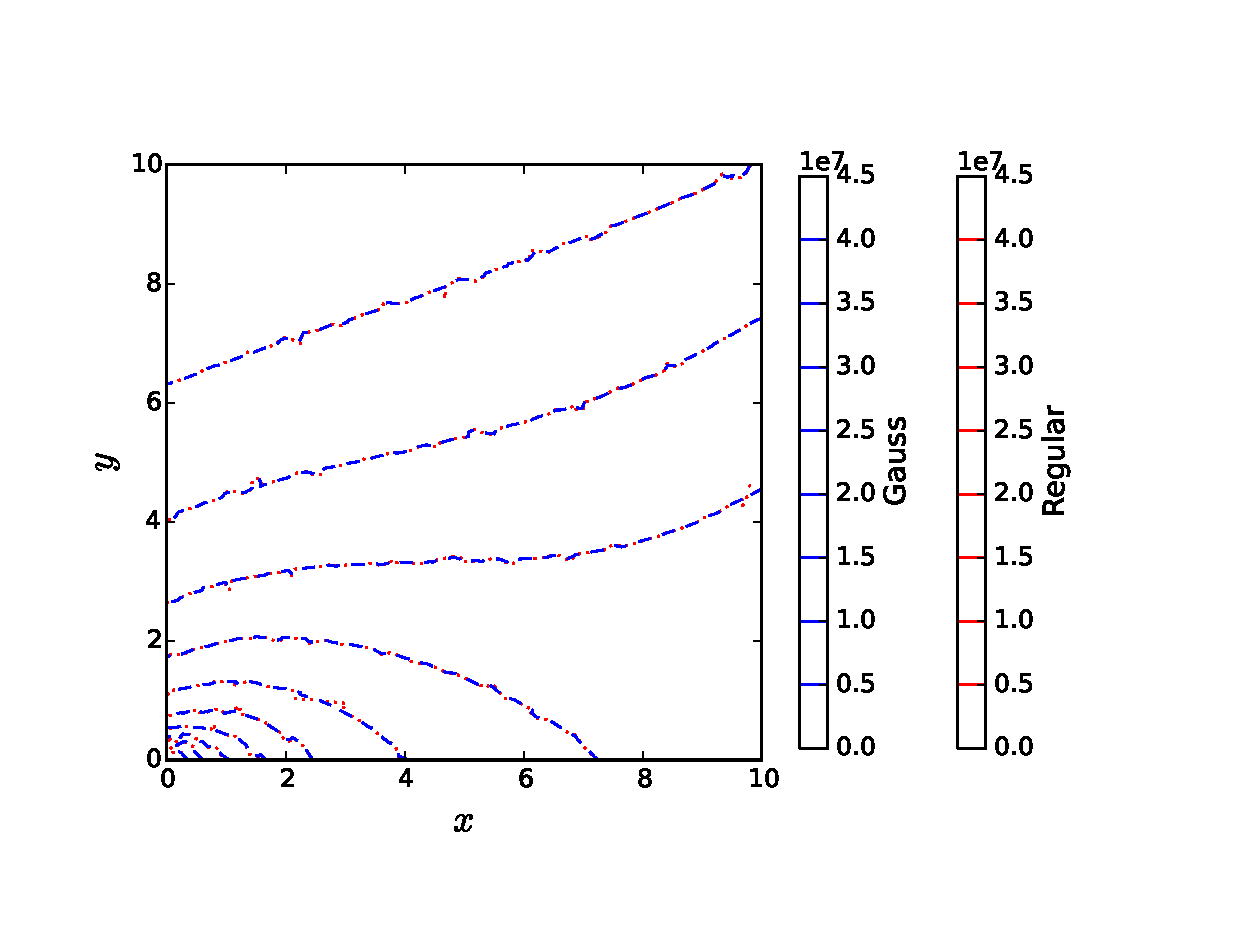
\includegraphics[width=0.8\textwidth]{fig/gauss_x_regular.eps}
		\caption{}
		\label{fig:1}
	\caption{Differences between stress recovery from nodal points and from Gauss points.}
	\label{fig:3_1}
\end{figure}


\end{document}
